
%\documentclass[conference,letterpaper,10pt]{IEEEtran}
\documentclass[journal,draftcls,onecolumn,12pt,twoside]{IEEEtran}
\newcommand{\folder}{/home/bohulu/Documents/texmf}
%\newcommand{\folder}{/home/hanchenggao/Documents/texmf}
\input{\folder/hfiles/epaper}
%\renewcommand{\thesubsubsection}{\Alph{subsubsection}.}
%\setcounter{secnumdepth}{3}
%\usepackage[ruled,vlined]{algorithm2e}
\usepackage {graphics}
\usepackage{caption}
\usepackage{tabularx}
%\usepackage {graphics}
%\setCJKmainfont{SimSun}
\begin{document}
\title{
A Novel Method for Obtaining the Pattern of Low-Weight Codeword Components of Recursive Systematic Convolutional Codes}
\author{%
  \IEEEauthorblockN{Bohulu~Kwame~Ackah~and~Chenggao~Han\\}four
  \IEEEauthorblockA{Graduate School of Informatics and Engineering,\\
   The University of Electro-Communications,\\
    1-5-1 Chofugaoka, Chofu-shi, Tokyo, 182--8585, Japan\\
                    Email: \{bohulu, han.ic\}@uec.ac.jp}
}
%\author{Bohulu~Kwame~Ackah~and~Chenggao~Han
%\thanks{K. A. Bohulu and C. Han are with the Graduate School of Informatics and Engineering, The University of Electro-Communications, 1-5-1 Chofugaoka, Chofu-shi, Tokyo, 182--8585, Japan, Email: \{bohulu, han.ic\}@uec.ac.jp}}
%\markboth{Journal of \LaTeX\ Class Files,~Vol.~14, No.~8, August~2015}%
%{Shell \MakeLowercase{\textit{et al.}}: Bare Demo of IEEEtran.cls for IEEE Journals}


\maketitle
\begin{abstract}
%Knowledge of the distance spectrum, as well as the structure of the message inputs that make up the distance spectrum for a specific recursive systematic convolutional (RSC) code is vital to the design of Turbo Code interleavers. Even though the distance spectrum of an RSC code can be obtained by calculating its transfer function, it does not provide any information about the structure of the message inputs. %and the complexity involved in calculating the transfer function increases with the number of states of the RSC code.
%%%%%%%%%%%%%%%%%%%%%%%%%%%

In this paper, we present a novel low-complexity method for determining the pattern of the low-weight codeword components of any RSC code as well as the distance spectrum. 
Using our method, we list the partial distance spectrum for selected RSC codes up to a cut-off weight $d_{\text{max}}$ and compare the simulation results to the bounds obtained via our novel method and the transfer function method. 
\end{abstract}
\newpage
\section{Introduction}

The {\it turbo code} (TC) \cite{ref1} is one of the forward-error correcting codes that comes very close to satisfying the Shannon limit for AWGN channels. It was introduced by Claude Berrou in 1993 and has been used in many applications and it has been adopted as the channel code for the LTE standard, IEEE 802.16 WiMAX (worldwide interoperability for microwave access) and DVB-RCS2 (2nd generation digital video broadcasting - return channel via satellite) standards \cite{ref7}.

 The simplest and most common construction of a TC is the parallel concatenation of two {\it recursive systematic convolutional} (RSC) codes (usually of the same kind) via an interleaver. One of the many reasons why the TC excels as a channel code is its ability to map low-weight parity-check sequences in the first component RSC code to high-weight parity-check sequences in the second component RSC code using an interleaver, which in turn generates TCs with a large minimum distance value and low multiplicity.
%The reason why the TC has such a good error correcting capability has been attributed to the low multiplicity of its minimum distance codeword and through many years of intensive research in the field, it is common knowledge that this is largely due to the use of the interleaver in the TC construction.

 For this reason, interleaver design for TCs has been highly researched for many years and generally, they are grouped into random and deterministic interleavers. Random interleavers determine their order of permutation in a pseudo-random manner. TCs using random interleavers usually have good error-correcting capabilities but impose huge memory constraints for many practical applications due to the use of interleaver tables. A notable example of a random interleaver is the S-random interleaver.
% and therefore require interleaver tables in both the transmitter and the receiver. Even though TCs made with random interleavers have very good error-correcting capabilities (especially for medium and long frame sizes), the need for interleaver tables imposes huge memory constraints for many practical applications. A notable example of a random interleaver is the S-random interleaver.

On the other hand, deterministic interleavers generate their order of 
permutation via \newline algorithms and as such, can be generated on the fly, and do not require permutation tables. 
Popular deterministic interleavers include \textit{quadratic permutation polynomial} (QPP) interleaver \cite{ref5}, \textit{almost regular permutation} (ARP) interleaver \cite{ref6} and \textit{dithered relative prime} (DRP) interleaver. A protograph based interleaver design for punctured turbo codes is also introduced in \cite{ref7}. 
Deterministic interleavers also make it possible to perform parallel decoding once the interleaver meets certain requirements. Despite all these benefits, it is a well-known fact that in terms of TC error-correcting performance, random interleavers always outperform deterministic interleavers, especially for long frame sizes.
%Another benefit of using deterministic interleavers is the ability to custom design the interleaver to a specific component code to improve the overall error-correcting capability of the TC. 

%The most common approach to deterministic interleaver design is the minimum free distance ($d_{\text{free}}$) maximisation approach, where the interleaver is designed with the aim of maximising the value of $d_{\text{free}}$. This approach, while simplistic, has produced some good interleavers only after considering higher weight inputs \cite{ref5}. Therefore,
%using it as a general rule of thumb for all deterministic interleaver design approaches might not be the best, especially when the minimum distance codeword for the component code is generated by an input message with a weight greater than 2. 
The design of a good deterministic interleaver requires the complete knowledge of all the low-weight codeword patterns in the component RSC codes and missing even one of these patterns can result in deterministic interleavers that generate TCs with sub-par error correction performance.
The transfer function of an RSC code is an interleaver design tool that provides information about the different weights in the code, as well as their corresponding multiplicities (distance spectrum). However, it provides no information with regards to the pattern of the low-weight codewords. As an added downside, the complexity of calculating the transfer function for a given RSC code increases with the number of states. To the best of our knowledge, there exists no interleaver design tool that provides knowledge of both the distance spectrum and the low-weight codeword patterns. Because of this, many of the interleaver design methods end up completely ignoring certain important low-weight codewords. In \cite{ref5} for example, the interleaver design method does not take into account the existence of low-weight codewords generated by message inputs of weight 3, especially for the $5/7$  RSC code, where such codewords are very dominant.

In this paper, we present a novel method that can be used to find the distance spectrum of an RSC code as well as the pattern of the low-weight codewords. The complexity of our method is independent of the number of states of the RSC code and its ability to reveal low-weight codeword patterns of an RSC code makes it an excellent tool for use in interleaver design.

In order to validate our method, we generate a partial distance spectrum for specific RSC codes and compare it to the lower bound obtained via the transfer function method. We also compare the bounds obtained using our novel method to simulation results. In both cases, it is observed that the values begin to converge as $E_b/N_0$ increases.

The remainder of the research paper is organised as follows. Notations and definitions used in the research paper are introduced in Section \ref{secPrelim}. In Section \ref{sec2}, we briefly review the RSC codes. Moving on to Section \ref{sec3}, we present the theory behind our novel method and use it to generate a partial distance spectrum using a union bound-like approach for selected RSC codes in \ref{sec4}. Comparison of bounds obtained using our novel method to that obtained using the transfer function as well as  simulation results are presented in Section \ref{sec5} and the paper concludes in Section \ref{sec6}.
\newpage
\section{Preliminaries}
\label{secPrelim}
$v(x)$ denotes the polynomial representation of any binary sequence. 
Specifically, the symbols $b(x)$ and $h(x)$ represent the input message and parity-check sequence respectively in polynomial form. 
The Hamming weight of $b(x)$ and $h(x)$, denoted by $w_H(b(x))$ and $w_H(h(x))$ respectively, is equal to the length of the polynomial $b(x)$ or $h(x)$.

$m$ is used to represent the order of $v(x)$ and GF($2^{m}$) represents the extended Galois field generated by a prime polynomial which has order $m$.
$\beta^i$ represents a non-zero element in  GF($2^{m}$), $1 \leq i \leq 2^m-1$.
Any $\beta^i \st (\beta^i)^j=1,~j\leq 2^m-1$ is know as a \textit{primitive element}

Given a pair of integers $(e,~f)$, $(e,~f) \bmod 2^m-1$ is shorthand for the operation $(e \bmod 2^m-1,~f \bmod 2^m-1)$.


% an infinite repetition of the vector $\bv$ whiles $(\bv)_j$ represents the repetition of vector $\bv~j$ times   

%$\bphi$ represents a primitive element in the extended Galois field GF($2^{\tau}$) and the vector representation for all elements in GF($2^{\tau}$) are written as $\bphi_i,~0 \leq i \leq 2^{\tau}$. 

%The subscript $i$ represents the decimal value of the binary vector, which means $\bphi_0$ represents the all-zero vector. All addition and multiplication operations are done in GF($2^{\tau}$).

%The operation $(e \bmod M,~f \bmod M)$ is represented by $(e,~f) \bmod M$, where $(e,~f)$ are integer pairs.

\newpage
\section{Union Bound of RSC Codes}
\label{sec2}
The outputs of an RSC code are determined by the input bit sequence $b(x)$, the states of the shift registers and the feedforward and feedback connections of shift registers that can be represented by a generator function. 

As an instance,  the generator function of a rate $1/2$ RSC code may be written as  $$\Big[1 ~\frac{f(x)}{g(x)}\Big]$$ where $1$ yields the \textit{systematic  component} (SC) $b(x)$ while the \textit{parity-check component} (PC) $h(x)$ is associated with the feedforward and feedback connections of the shift registers, specified by  $f(x)$ and $g(x)$, respectively. The outputs $c(x)$ are a mixture of SC and PC as
\begin{equation}
c(x) = b(x^2)+xh(x^2)
\label{codeword-comp}
\end{equation}
where 
\begin{equation}
h(x) =f(x)g^{-1}(x)b(x)
\label{eq:parity-def}
\end{equation}
From \eqref{codeword-comp}, we have
\begin{equation}
w_H(c(x))=w_H(b(x)) + w_H(h(x))
\label{eq:cw-weight}
\end{equation}
 and it is obvious that each low-weight codeword is a conjunction of two low-weight SC and PC.

Under the assumption of large frame sizes, the presence of $g^{-1}(x)$  in \eqref{eq:parity-def} may involve a particular sequence of bits that is repeated a large number of times, hence a high-weight PC. A low-weight PC occurs if and only if
\begin{equation}
b(x) \bmod g(x) \equiv 0
\label{eq:rtz-input}
\end{equation}
and the inputs $b(x)$ which meet the condition in \eqref{eq:rtz-input} is called a \textit{return-to-zero} (RTZ) input. Thus, every RTZ input can be factorized by  
\begin{equation}
b(x) =a(x)g(x)
\label{eq:low-weight-msg}
\end{equation}
where $a(x)$ is a monic polynomial, $a_0=1$.
Substituting (\ref{eq:low-weight-msg}) into \eqref{eq:parity-def}, we can characterize the low-weight PC as
\begin{equation}
\begin{split}
h(x)&=f(x)\cdot g^{-1}(x)\cdot a(x)g(x)\\
&=a(x)f(x)
\end{split}
\label{eq:low-weight-parity}
\end{equation}
%(quarantine)%Using both (\ref{novelEq2})  and (\ref{novelEq3}), we wish to list all low-weight codewords for a given RSC code.A low-weight codeword is any codeword which satisfies the condition, $w_H(\bc) \leq d_{\text{max}}$. This list is known as the \textit{partial structured distance spectrum}. To generate the partial structured distance spectrum, we take note of a few things. 

%From (\ref{novelEq2})  and (\ref{novelEq3}), we observe that $a(x)$ is a common factor in both equations and if we are able to solve for $a(x)$ via either of the equations, the remaining equation can be solved. To solve for $a(x)$ requires that in either equation, it should be the only unknown variable. At first glance, it might seem that $g(x)$ and $f(x)$ are the only known variables because they are dependent on the RSC code in question. However, if we remember that the weight of $h(x)$ and $b(x)$ is directly proportional to the number of terms it has, then we are on our way to obtain our second known variable. What is left is to determine the valid power values for the polynomial  terms, depending on the weight of $h(x)$ or $b(x)$.

Finally, for a given RSC code, we can formulate our goal as, to find all $a(x)$s which satisfy  \eqref{eq:low-weight-msg} and  \eqref{eq:low-weight-parity} simultaneously. However, since there is essentially no difference between the two equations, in the next section, we oresent a method for determining the low-weight PC patterns for $2 \leq w_H(h(x)) \leq 3$


 %an RSC encoder which takes in $k$ bits and outputs $n$ bits at every time instance.The output bits of an RSC code are generated using the feedforward and feedback connections of shift registers determined by its generator function. The generator function may be written in polynomial notation as $\Big[1 ~\frac{f(x)}{g(x)}\Big]$, where $1$ yields the systematic (input) part  of the output while the parity check part of the output are specified by  $f(x)$ and $g(x)$ that represent the feedforward and feedback connections of the shift registers respectively. Through out this paper, $c(x),~b(x)$ and $h(x)$ represesent the RSC codeword, the systematic component of the codeword and the parity check component of the codeword, respectively in polynomial notation.

%\subsection{Low-weight Components}
%(quarantine)%The distance spectrum derived via the transfer function method is an insufficient tool when it comes to to interleaver design. In this section, we present a novel method that generates what we refered to as the structured distance spectrum, which is the distance spectrum with the structure of the RTZ inputs as well as the corresponding parity-check sequence revealed, therefore making it a very useful tool for interleaver design.

%(quarantine)%For an RSC code, the Hamming weight of the codeword $w_H(\bc)$ is the sum of the weights of the parity bit sequence and message input. 
The parity-check sequence can be expressed as 
\begin{equation}
h(x) =f(x)\cdot g^{-1}(x)\cdot b(x)
\label{novelEq0}
\end{equation}
If we consider large frame sizes, the presence of $g^{-1}(x)$ means that within $h(x)$ is a particular sequence of bits that is repeated a large number of times. This results in a large parity weight, and by extension, a relatively high-weight codeword. The only time this is not the case is when
\begin{equation}
b(x) \bmod g(x) \equiv 0
\label{novelEq1}
\end{equation}
This results in a relatively low-weight parity bit sequence, which might produce a low-weight codeword. Any $b(x)$ that meets the condition in (\ref{novelEq1}) can be written as 
\begin{equation}
b(x) =a(x)g(x)
\label{novelEq2}
\end{equation}
where $a(x)$ is a monic polynomial with the coefficient of the lowest term not equal to $0$.
By fixing $b(x)$ from (\ref{novelEq2}) into (\ref{novelEq0}), we have 
\begin{equation}
\begin{split}
h(x)&=f(x)\cdot g^{-1}(x)\cdot a(x)g(x)\\
&=a(x)f(x)
\end{split}
\label{novelEq3}
\end{equation}
%(quarantine)%Using both (\ref{novelEq2})  and (\ref{novelEq3}), we wish to list all low-weight codewords for a given RSC code.A low-weight codeword is any codeword which satisfies the condition, $w_H(\bc) \leq d_{\text{max}}$. This list is known as the \textit{partial structured distance spectrum}. To generate the partial structured distance spectrum, we take note of a few things. 

%From (\ref{novelEq2})  and (\ref{novelEq3}), we observe that $a(x)$ is a common factor in both equations and if we are able to solve for $a(x)$ via either of the equations, the remaining equation can be solved. To solve for $a(x)$ requires that in either equation, it should be the only unknown variable. At first glance, it might seem that $g(x)$ and $f(x)$ are the only known variables because they are dependent on the RSC code in question. However, if we remember that the weight of $h(x)$ and $b(x)$ is directly proportional to the number of terms it has, then we are on our way to obtain our second known variable. What is left is to determine the valid power values for the polynomial  terms, depending on the weight of $h(x)$ or $b(x)$.

In (\ref{novelEq3}), once $f(x)$ is given, our goal is to find $a(x)$ that results in a low-weight $h(x)$. To this end, we consider the roots of $f(x)$ 
%If $f(x)$ is a prime polynomial or can be factorized into prime polynomials, the the roots of $f(x)$ are its primitive elem
 %denoted by $\beta_i,~ 0 \leq i < 2^{m}-1)$. Then it is obvious that $h(\beta^i)=0$~ for all $\beta^i$ that are primitive elements 
and we can reformulate our goal as to find weight-$w$ polynomials ($h(x)$) which take all the roots of $f(x)$ as its roots. The roots of $f(x)$ depend on its characteristic make-up and once that is known, we can easily determine the structure of $h(x)$ for a given value of $w_H(h(x))$. 
The characteristic make-up of $f(x)$ can be grouped into the three cases below. 
\begin{enumerate}
\item Single primitive polynomial.
\item Prime but not a primitive polynomial.
\item Made up of repeated polynomial roots.
\end{enumerate}
We present a method for determining valid values of $h(x)$ for a given RSC code when $2 \leq w_H(h(x))\leq 3$. 

It is worth noting that the method to be discussed can also be used to obtain valid values of $b(x)$, because there is no difference between the general structure of $h(x)$ and $b(x)$ once the Hamming weight is fixed. 
%\section{ Codeword Component Pattern List and the Union Bound }
\label{sec4}
%For a given RSC code, the distance spectrum provides information concerning the multiplicity of a codeword for a fixed weight and it is an effective tool to evaluate its error-correcting capability. In practice however, since higher-weight codewords have very little effect on its overall error-correcting capability, we usually use a partial distance spectrum, where the largest codeword weight value is set to $d_{\text{max}}$. 

%The distance spectrum of the RSC code can be obtained from its transfer function, denoted by $$T(Y,X)=\sum_{d=0}^{\infty}\sum_{w=0}^{\infty} a(d,w)Y^dX^w$$ where $a(d,w)$ is the number of codewords of weight $d$ generated by an input bit sequence of weight $w$. 
%The transfer function enumerates all the paths that diverge from and then return to the initial state \cite{ref3}, \textit{i.e.} the RTZ input paths. 
%Once the transfer function of an RSC code is known, it can be used to obtain bounds on the error-correcting capability using the union bound.
%Unfortunately, the complexity involved in deriving the transfer function increases as the number of states of the RSC code increases and other methods such as Mason's Rule \cite{ref3} have to be used. 

%For a given RSC code, we have shown in \ref{subsec:low-weight} that each codeword $c(x)$ is made up of $b(x)$ and $h(x)$ which have $a(x)$ as their common factor as shown in (\ref{novelEq2}) and (\ref{novelEq3}).
In this section, we outline our method for obtaining the list of all low weight codewords for a given RSC code.

 Let $\cA_h(d)$ be the set of all $a(x)$ which yields weight-$d$ parity-check component \ie, $w_H(h(x))=w_H(a(x)f(x))=d$ for $a(x) \in \cA_h(d)$. 
Similarly $\cA_b(d)$ is the set of all $a(x)$ which yields weight-$d$ systematic component \ie, $w_H(b(x))=w_H(a(x)g(x))=d$ for $a(x) \in \cA_b(d)$
 and $\cA_c(d)$ is the set of all $a(x)$ which yields weight-$d$ codeword \ie, $w_H(c(x))=w_H(a(x)f(x))+ w_H(a(x)g(x))=d$ for $a(x) \in \cA_c(d)$.  

From \eqref{eq:cw-weight}, when $w_H(b(x)), w_H(h(x)) \geq 2$, we have
\begin{align}
\cA_c(d) = \bigcup_{\ell = 2}^{d-2} \left\{\cA_b(\ell) \cap \cA_h(d-\ell)\right\}
\label{Eq:exactset}
\end{align}
However, to determine $\cA_b(\ell)$ or $\cA_h(\ell)$ for a large $\ell$ is a complex task in general. Thus, in this paper, we replace the set $\cA_c(d)$ by the approximated set $\cA_c'(d)$ as defined in  (\ref{setApprox})
\begin{equation}
\begin{split}
\cA_c(d) \approx \cA_c'(d) &= \left\{\bigcup_{\ell = 2}^{\ell+\alpha} \left\{\cA_b(\ell) \cap \cA_h(d-\ell)\right\}\right\}\bigcup \\
&\left\{\bigcup_{\ell = 2}^{\ell+\alpha} \left\{\cA_b(d-\ell) \cap \cA_h(\ell)\right\}\right\}
\end{split}
\label{setApprox}
\end{equation}
where some codewords in $\cA_c(d)$ with $\ell \approx d-\ell$ may be ignored in $\cA_c'(d)$.
%We refer to the distance spectrum obtained using this method as the \textit{codeword component pattern distance spectrum}
\begin{example}
If we set $d=8$ and  $\alpha=1$, $\cA_c'(8)$ becomes
\begin{equation*}
\begin{split}
\cA_c'(8) &=\left\{\left\{\cA_b(2) \cap \cA_h(6)\right\} \bigcup  \left\{\cA_b(3) \cap \cA_h(5)\right\} \right\} \bigcup \\
& \left\{\left\{\cA_b(6) \cap \cA_h(2)\right\} \bigcup  \left\{\cA_b(5) \cap \cA_h(3)\right\} \right\} \\
\end{split}
\end{equation*}

We can see that $\left\{\cA_b(4) \cap \cA_h(4)\right\}$ is not used in $\cA_c'(8)$, event though it is used in $\cA_c(8)$.
\end{example}
Once we obtain the set
 \begin{equation*}
 \bigcup_{d = d_{\text{min}}}^{d_{\text{max}}} \cA'_c(d) 
\label{Eq:exactsetunion}
\end{equation*}
, we can list the low weight codeword component patterns for a given RSC code using \eqref{eq:low-weight-msg} and \eqref{eq:low-weight-parity}.  We set $d_{\text{max}}=d_{\text{min}}+3$ and  list the low weight codeword component patterns for the $5/7,~37/21$ and $23/35$ RSC codes in Tables \ref{novelTab13},  \ref{novelTab14} and \ref{novelTab15} respectively. 

\begin{table}[htbp]
 \caption{Partial Codeword Component Pattern Distance Spectrum for the $5/7$ RSC code, $d_{\text{free}}=5$}
\centering
 \begin{tabularx}{0.45\textwidth}{XlX} 
 \hline
 $a(x)$ & $b(x)$ & $h(x)$ \\ %[0.5ex] 
 \hline\hline
$1$ & $1+x+x^{2}$ & $1+x^2$\\
\hline
$1+x^2$ & $1+x+x^3+x^4$ & $1+x^{4}$\\
\hline
$1+x$ & $1+x^3$ & $1+x+x^2+x^3$\\
\hline
$1+x^2+x^4$ & $1+x+x^3+x^5+x^6$ & $1+x^{6}$\\
\hline
$1+x^2+x^3$ & $1+x+x^5$ & $1+x^3+x^4+x^5$\\
\hline
$1+x+x^2$ & $1+x^2+x^4$ & $1+x+x^3+x^4$\\
\hline
$1+x+x^3$ & $1+x^4+x^5$ & $1+x+x^2+x^5$\\
\hline
$1+x^2+x^4+x^6$ & $1+x+x^3+x^5+x^7+x^8$ & $1+x^8$\\
\hline
$1+x+x^3+x^4$ & $1+x^6$ & $1+x+x^2+x^4+x^5+x^6$\\
%======extra
%\hline
%$1+x+x^3+x^5$ & $1+x^4+x^6+x^7$ & $1+x+x^2+x^7$\\
%\hline
%$1+x+x^2+x^4$ & $1+x^2+x^5+x^6$ & $1+x+x^3+x^6$\\
%\hline
%$1+x+x^2+x^3$ & $1+x^2+x^3+x^5$ & $1+x+x^4+x^5$\\
%\hline
%$1+x^2+x^3+x^5$ & $1+x+x^6+x^7$ & $1+x^3+x^4+x^7$\\
%\hline
%$1+x^2+x^3+x^4$ & $1+x+x^4+x^6$ & $1+x^3+x^5+x^6$\\
%\hline
%$1+x^2+x^4+x^5$ & $1+x+x^3+x^7$ & $1+x^5+x^6+x^7$\\
 \end{tabularx}
 
 \label{novelTab13}
\end{table}

\begin{table}[htbp]
 \caption{Partial Codeword Component Pattern Distance Spectrum for the $37/21$ RSC code, $d_{\text{free}}=6$}
\centering
 \begin{tabularx}{0.45\textwidth}{XlX} 
 \hline
 $a(x)$ & $b(x)$ & $h(x)$ \\ [0.5ex] 
 \hline\hline
$1+x$ & $1+x+x^{4}+x^5$ & $1+x^5$\\
\hline
$1$ & $1+x^4$ & $1+x+x^2+x^3+x^4$\\
\hline
$1+x+x^5+x^6$ & $1+x+x^4+x^6+x^9+x^{10}$ & $1+x^{10}$\\
%\hline
%$1+x+x^4+x^5$ & $1+x+x^8+x^9$ & $1+x^4+x^5+x^9$\\
%\hline
%$1+x^2$ & $1+x^2+x^4+x^6$ & $1+x+x^5+x^6$\\
%\hline
%$1+x+x^5$ & $1+x+x^4+x^9$ & $1+x^6+x^7+x^8+x^9$\\
%\hline
%$1+x+x^4$ & $1+x+x^5+x^8$ & $1+x^4+x^6+x^7+x^8$\\
%\hline
%$1+x^2+x^4$ & $1+x^2+x^6+x^8$ & $1+x+x^4+x^7+x^8$\\
%\hline
%$1+x^3+x^4$& $1+x^3+x^7+x^8$ & $1+x+x^2+x^4+x^8$\\
%\hline
%$1+x^4+x^5$ & $1+x^5+x^8+x^9$ & $1+x+x^2+x^3+x^9$\\
 \end{tabularx}
 
 \label{novelTab14}
\end{table}

\begin{table}[htbp]
 \caption{Partial Codeword Component Pattern Distance Spectrum for the $23/35$ RSC code, $d_{\text{free}}=7$}
\centering
\begin{tabularx}{0.45\textwidth}{XlX} 
 \hline
 $a(x)$ & $b(x)$ & $h(x)$ \\ [0.5ex] 
 \hline\hline
$1+x^2+x^3$ & $1+x^7$ & $1+x+x^2+x^6+x^7$\\
\hline
$1$ & $1+x^2+x^3+x^4$ & $1+x+x^{4}$\\
\hline
$1+x+x^2+x^3+x^5$ & $1+x^3+x^4+x^8+x^9$ & $1+x^7+x^9$\\
\hline
$1+x+x^2+x^3+x^5+x^7+x^8$ & $1+x+x^3+x^4+x^7+x^{12}$ & $1+x^{11}+x^{12}$\\
\hline
$1+x^2+x^3+x^7+x^9+x^{10}$ & $1+x^{14}$ & $1+x+x^2+x^6+x^8+x^9+x^{13}+x^{14}$\\
 \end{tabularx}
 
 \label{novelTab15}
\end{table}

%Having determined how to find valid values of $b(x)$ and $h(x)$ for Hamming weights $\leq 3$, we are now in a position to generate the codeword pattern distance spectrum for a given RSC code. We take a union bound like approach towards the generation of the codeword pattern distance spectrum. The approach is outlined below.
%\begin{enumerate}
 %\item Beginning with (\ref{novelEq2}), we find all values of $b(x),~w_H(b(x))=2$ that have the same roots as $g(x)$ and divide $g(x)$ by each valid polynomial to obtain the corresponding $a(x)$.\label{ubStep1}
 %\item Then using (\ref{novelEq3}), we multiply each $a(x)$ by $f(x)$ to obtain the corresponding value of $h(x)$. It is worth noting that $w_H(h(x))$ may be $\geq w_H(b(x))$. \label{ubStep2}
 %\item Since we are interested in only the low weight codewords, we ignore any $b(x) \st w_H(b(x))+w_H(h(x)) \geq d_{\text{max}}$. \label{ubStep3}
 %\item Next we set the weight value of $b(x)$ to $w_H(b(x))=3$, and repeat steps \ref{ubStep1} and \ref{ubStep2} while ignoring $b(x)$ that meet the condition in step \ref{ubStep3}.\label{ubStep4}
 %\item To obtain a complete codeword pattern distance spectrum, we do a reverse operation, \textit{i.e.} we focus on (\ref{novelEq2}) and find all values of $g(x),~w_H(\bh)=2$ that have the same roots as $f(x)$ and divide $f(x)$ by each valid polynomial to obtain the corresponding $a(x)$.
 %\item Then using (\ref{novelEq2}), we repeat steps \ref{ubStep2} through \ref{ubStep4}, being careful to avoid repitition.
 %\item Finally we arrange all valid values of $b(x)$ and $h(x)$ in ascending value of codeword weight,$w_H(b(x)) + w_H(h(x))$.
 %\end{enumerate}

%We use the codeword pattern distance spectrum to calculate the bit-error bounds for each RSC and compare them to the bit-error bounds obtained via the distance spectrum as well as simulation results. We use the probability of bit-error in doing this and a more general formula for calculating $P_b$ is shown below [4]:

%\begin{equation}
%P_b \leq \frac{1}{k} \sum_{d=d_{\text{free}}}^{\infty} w(d) Q\Bigg( \sqrt{\frac{2dE_c}{N_0}}\Bigg)
%\label{novelEq6}
%\end{equation}
%where $w(d)=\sum_{i=1}^{\infty} i~ a(d,i)$ and $ a(d,i)$ is the number of codewords of weight $d$ generated by an input message of weight $i$. If we set a limit on the maximum value of the codeword weight $d_{\text{max}}$
% we can rewrite (\ref{novelEq6}) as 
%\begin{equation}
%P_b \leq \frac{1}{k} \sum_{d=d_{\text{free}}}^{d_{\text{max}}} w(d) Q\Bigg( \sqrt{\frac{2dE_c}{N_0}}\Bigg)
%\label{novelEq7}
%\end{equation}
 %From the simulation results, we observed $d_{\text{max}}=d_{\text{min}}+3$ is a sufficient value for obtaining the BER bounds.
%In order to confirm the validity of our method, we use the values obtained from Tables \ref{novelTab8}, \ref{novelTab9} and \ref{novelTab10} to find the bounds for the BER of the RSC code, $P_b$.Finally, we compare the results obtained to $P_b$ found using the Transfer Function method as well as the simulation results.


In order to validate our novel method, we can calculate the lower bound for each RSC code by modifying the union bound of the bit-error rate
equation in \cite{ref4}, which gives us 
%\begin{align}
%P_b \leq \frac{1}{k} \sum_{d=d_{\text{free}}}^{\infty} \sum_{a(x) \in \cA_c(d)}w_H(a(x)g(x)) Q\Bigg( \sqrt{\frac{2dE_c}{N_0}}\Bigg)
%\label{novelEq6-1}
%\end{align}
%However, since the high-weight codewords have minor contribution on the unioin bound, \eqref{novelEq6-1} can be further approximated by setting a limit on the maximum value of the codeword weight $d_{\text{max}}$, resulting in
\begin{align}
P_b \leq \frac{1}{k} \sum_{d=d_{\text{free}}}^{d_{\text{max}}} \sum_{a(x) \in \cA'_c(d)}w_H(a(x)g(x)) Q\Bigg( \sqrt{\frac{2dE_c}{N_0}}\Bigg)
\label{novelEq7}
\end{align}
\newpage
%The minimum distance ($d_{\text{min}}$) of the RSC code determines its error-correcting capability. With the aid of the distance spectrum, it is possible to determine $d_{\text{min}}$ as well as its multiplicity. The most common way to find the distance spectrum is via the transfer function of the RSC code. The transfer function enumerates all the paths that diverge from and then return to the initial state \cite{ref3}, \textit{i.e.} the RTZ inputs. In other words, the distance spectrum provides information about the number of codewords of weight $d$ generated by an RTZ input of weight $w$. 

%Also to obtain the distance spectrum requires an extra division operation. In the case of interleaver design for turbo codes, this method for generating the distance spectrum is not particularly useful. This is because it reveals no extra details with respect to the structure of the RTZ inputs. 
%Next, we present our novel method, whose complexity is independent of the number of states in the RSC code. As an added bonus, information regarding the structure of the RTZ inputs can be obtained using this method.

%\begin{figure}[h]
%\centering
%		\includegraphics[width=0.45\textwidth]{./PaperSources/RSCExample3.pdf}
	%	\caption{$[\frac{1+x^2}{1+x+x^2}]$  RSC Encoder}
		%\label{fig1}
		%\end{figure}

%\begin{example}		
%An RSC encoder is shown in Figure \ref{fig1} with $k=1$ and $n=2$. Its parity generator\newline function is given by $[\frac{1+x^2}{1+x+x^2}]$, which may be written as $5/7$ in octal form, where $5 ~ \text{and} ~ 7$ correspond to the numerator and denominator of the generator function, respectively. 
 %For this RSC code, the cycle is $\bphi_g=\bphi_6 $ with a cycle length $\tau =3$. While $\bphi=(1~1~1~ 0~ 1~ 1~ 0~ 1~ 1~ 0~\cdots)$, which may be written in terms of the elements of GF(8) as $\bphi_7~\dot{\bphi_3}$ represents the impulse response. 
 %\end{example}
 % Moving forward all other examples and discussions relating to RSC codes will be done using the $5/7$ RSC code unless otherwise stated.

 %The knowledge of $\textbf{p}$ and $\tau$ will be used in deriving the method for determing which input messages generate low-weight parity bits. 
\newpage
%\begin{example}$f(x)=1+x+x^2$.\newline 

\textbf{Weight-2 PCs}: 
For this case, since $x^1=x$, $x^2 \equiv 1+x$, and $x^3 \equiv 1 \bmod f(x)$, the order of the root $\beta_0$ is $\epsilon_0=3$ and $a$ should be a multiple of $3$. The corresponding values for $a(x)$ and $h(x)$ are shown in Table \ref{novelTab2} for the first four valid values of $a$.
\begin{table}[htbp]
%\parbox{.5\linewidth}{
 \caption{$f(x)=1+x+x^2$}
\centering
 \begin{tabular}{c c c} 
%\hline
 $a(x)$ & $h(x)$ \\ [0.5ex] 
 \hline\hline
$1+x$
 & $1+x^{3}$ \\
\hline
$1+x+x^3+x^4$
 & $1+x^{6}$ 
 \\
\hline
$1+x+x^3+x^4+x^6+x^{7}$ 
&  $1+x^{9}$ 
\\
\hline
$1+x+x^3+x^4+x^6+x^{7}+x^9+x^{10}$
 &  $1+x^{12}$ \\
 \end{tabular}
 \label{novelTab2}
\end{table}
\label{ex-2}

We may write the weight-2 PCs in general form as $h(x)=1+x^{3\ell},~\ell>1$ and the corresponding $a(x)$ is given by 
\begin{equation*}
a(x)=\sum_{\ell=0}^{L-1} x^{3\ell}(1+x)
\end{equation*}

\textbf{Weight-3 PCs}: The elements of GF$(2^2)$ are shown in Table \ref{novelTab7} and it is obvious that $\cZ=\{(1,2)\}$.
This means that $(a,b) \in \{3\ell+1,~3n+2\},~l=n=\left\{0,1,...\right\}$.  The corresponding values for $a(x)$ and $h(x)$ are shown in Table \ref{novelTab8} below for the first four valid values of $(a,b)$.
 \begin{table}[htbp]
 \caption{Non-zero Elements of GF$(2^2)$ generated by $f(x)=1+x+x^2$}
\centering
 \begin{tabular}{c c} 
 \hline
 power representation & actual value \\ [0.5ex] 
 \hline\hline
$X^0~=X^3=1$ & $1$\\
\hline
$X$ & $x$\\
\hline
$X^2$ &  $1+x$\\
\hline
 \end{tabular}
 \label{novelTab7}
\end{table}

\begin{table}[htbp]
 \caption{$f(x)=1+x+x^2$}
\centering
 \begin{tabular}{c c} 
 \hline
 $a(x)$ & $h(x)$\\ [0.5ex] 
 \hline\hline
$1$ & $1+x+x^2$\\ 
\hline
$1+x+x^2$ &  $1+x^2+x^4$\\
\hline
$1+x+x^3$ & $1+x^4+x^5$\\
\hline
$1+x^2+x^3$ & $1+x+x^5$ 
 \end{tabular}
 \label{novelTab8}
\end{table}

We may write the weight-3 PCs in general form as $h(x)=1+x^{3\ell+1}+x^{3n+2},~\ell,~n \geq 0$ 

\label{ex-1}
\end{example}




\begin{example}
$f(x)=1+x+x^2+x^3+x^4$\newline

\textbf{Weight-2 PCs}: 
We can confirm that the order of $\beta_0$ is $\epsilon_0=5$. This means that $a$ should be a multiple of $5$. The corresponding values for $a(x)$ and $h(x)$ are shown in Table \ref{novelTab3} with general forms for $\ell>1$

%}
\begin{table}[htbp]
%\parbox{.5\linewidth}{
\caption{$f(x)=1+x+x^2+x^3+x^4$}
\centering
\begin{tabular}{c c} 
 \hline
 $a(x)=\sum_{\ell=0}^{L-1} x^{5\ell}(1+x)$ & $h(x)=1+x^{5\ell}$  \\ [0.5ex] 
 \hline\hline
$1+x$ &$1+x^5$\\ 
$1+x+x^5+x^6$ &$1+x^{10}$  \\
$1+x+x^5+x^6+x^{10}+x^{11}$ & $1+x^{15}$ \\
$1+x+x^5+x^6+x^{10}+x^{11}+x^{15}+x^{16}$ &$1+x^{20}$  
 \end{tabular}
 \label{novelTab3}
%}ll
\end{table}

\textbf{Weight-3 PCs}:
We refer to Table \ref{novelTabWt3-2} and it is obvious that $\cZ=\{ \}$ and therefore, there are no weight-3 PCs for $f(x)$
 \begin{table}[htbp]
 \caption{Non-zero Elements of GF$(2^4)$ generated by $f(x)=1+x+x^2+x^3+x^4$}
\centering
 \begin{tabular}{c c} 
 \hline
 power representation & actual value \\ [0.5ex] 
 \hline\hline
$X^0~=X^5~=X^{10}~=X^{15}$ & $1$\\
\hline
$X~=X^6~=X^{11}$ & $x$\\
\hline
$X^2~=X^7~=X^{12}$ &  $x^2$\\
\hline
$X^3~=X^8~=X^{13}$ &  $x^3$\\
\hline
$X^4~=X^9~=X^{14}$ &  $1+x+x^2+x^3$\\
\hline
 \end{tabular}
 \label{novelTabWt3-2}
\end{table}
\label{ex-2}
\end{example}

\begin{example}
	$f(x)=1+x^2$\newline
	
	\textbf{Weight-2 PCs}: Since 
	\[
	f(x)=(1+x)^2\]
	and the order of the root $\beta_0=1$ is $\epsilon_0=1$, we obtain from \eqref{Eq:rootcondition} and \eqref{Eq:differential}
	\begin{align}
		(\beta_0)^a = 1
		\label{Eq:example31}
	\end{align}
	\begin{align}
		a(\beta_0)^{(a-1)} = 0
		\label{Eq:example32}
	\end{align}	
	Although \eqref{Eq:example31} indicates $a$ can be any positive integer, we can see from \eqref{Eq:example32} that $a$ should be an even number.
	The corresponding values for $a(x)$ and $h(x)$ are shown in Table \ref{novelTab1} with general forms for $\ell>1$.
	\begin{table}[htbp]
		\renewcommand{\arraystretch}{1.3}
		%\parbox{.3\linewidth}{
		\caption{$f(x)=1+x^2$}
		\centering
		\begin{tabular}{c c } 
			\hline
			$a(x)=\sum_{\ell=0}^{L-1} x^{2\ell}$ & $h(x)=1+x^{2\ell}$ \\ [0.5ex] 
			\hline\hline
			$1$ & $1+x^2$\\ 
			$1+x^2$ & $1+x^4$ \\
			$1+x^2+x^4$ & $1+x^6$\\
			$1+x^2+x^4+x^6$ & $1+x^8$ 
		\end{tabular}
		\label{novelTab1}
	\end{table}
	
	\textbf{Weight-3 PCs}:
	Given that there is a single non-zero element in GF(2) which is generated by $1+x$ we can conclude that there are no weight-3 PCs associated with $f(x)$.
\label{ex-3}
\end{example}



---------------------------
%=====================Deleted Examples  =======================%
%\begin{example}
%$f(x)=1+x^2+x^3+x^4$\newline
%$f(x)$ can be written as 
%$$f(x)=\prod_{k=0}^{1}f_k(x)$$
%where 
%$$f_0(x)=1+x,~f_1(x)=1+x+x^3$$ 
%For $f_0(x), x \equiv 1$, and $x^1 \equiv 1 \bmod f_0(x)$, which means the order of the root $\beta_0$ is $\epsilon_0=1$ and $a_0$ should be a multiple of $1$. Again, for  $f_1(x), x^3 \equiv 1+x$, and $x^7 \equiv 1 \bmod f_1(x)$, which means the order of the root $\beta_1$ is $\epsilon_1=7$ and $a_1$ should be a multiple of $7$.
%Finally, valid values of $a$ should be a multiple of the least common multiples of $a_0$ and $a_1$, which means $a$ should be a multiple of $7$.
%The corresponding values for $a(x)$ and $h(x)$ are shown in Table \ref{novelTab1-a} with general forms for $\ell>1$.
%\begin{table}[htbp]
%\renewcommand{\arraystretch}{1.3}
%\parbox{.3\linewidth}{
 %\caption{$f(x)=1+x^2+x^3+x^4$}
 %\centering
%\begin{tabular}{c c } 
%\hline
 %$a(x)=\sum_{\ell=0}^{L-1} x^{7\ell}(1+x^2+x^3)$ & $h(x)=1+x^{7\ell}$ \\ [0.5ex] 
%\hline\hline
%$1+x^2+x^3$ & $1+x^7$\\ 
%$1+x^2+x^3+x^7+x^9+x^{10}$ & $1+x^{14}$ \\
%$1+x^2+x^3+x^7+x^9+x^{10}+x^{14}+x^{16}+x^{17}$ & $1+x^{21}$
%\end{tabular}
% \label{novelTab1-a}
%\end{table}
%\end{example}

%\begin{example}
%$f(x)=1+x+x^2+x^3+x^4+x^5+x^6$\newline
%$f(x)$ can be written as 
%$$f(x)=\prod_{k=0}^{1}f_k(x)$$
%where 
%$$f_0(x)=1+x^2+x^3,~f_1(x)=1+x+x^3$$ 
%For $f_0(x), x^3 \equiv x^2+1$, and $x^7 \equiv 1 \bmod f_0(x)$, which means the order of the root $\beta_0$ is $\epsilon_0=7$ and $a_0$ should be a multiple of $7$. Again, for  $f_1(x), x^3 \equiv 1+x$, and $x^7 \equiv 1 \bmod f_1(x)$, which means the order of the root $\beta_1$ is $\epsilon_1=7$ and $a_1$ should be a multiple of $7$.
%Finally, valid values of $a$ should be a multiple of the least common multiples of $a_0$ and $a_1$, which means $a$ should be a multiple of $7$.
%The corresponding values for $a(x)$ and $h(x)$ are shown in Table \ref{novelTab1-b} with general forms for $\ell>1$.
%\begin{table}[htbp]
%\renewcommand{\arraystretch}{1.3}
%\parbox{.3\linewidth}{
% \caption{$f(x)=1+x+x^2+x^3+x^4+x^5+x^6$}
 %\centering
%\begin{tabular}{c c } 
%\hline
 %$a(x)=\sum_{\ell=0}^{L-1} x^{7\ell}(1+x)$ & $h(x)=1+x^{7\ell}$ \\ [0.5ex] 
%\hline\hline
%$1+x$ & $1+x^7$\\ 
%$1+x+x^7+x^8$ & $1+x^{14}$ \\
%$1+x+x^7+x^8+x^{14}+x^{15}$ & $1+x^{21}$
%\end{tabular}
% \label{novelTab1-b}
%\end{table}
%\end{example}
%=====================================End of deleted examples========================%
\begin{example}
$f(x)=1+x^2+x^3+x^4+x^6$\newline

\textbf{Weight-2 PCs}: $f(x)$ can be written as 
$$f(x)=\prod_{k=0}^{1}f_k(x)$$
where 
$$f_0(x)=1+x+x^2,~f_1(x)=1+x+x^2+x^3+x^4$$ 
From Example \ref{ex-1} and Example \ref{ex-2}, we know that $a_0=3$ and $a_1=5$.
Hence, valid values of $a$ should be a multiple of the least common multiples of $a_0$ and $a_1$, which means $a$ should be a multiple of $15$.
The corresponding values for $a(x)$ and $h(x)$ are shown in Table \ref{novelTab1-c} with general forms for $\ell>1$.

\begin{table}[htbp]
\renewcommand{\arraystretch}{1.3}
%\parbox{.3\linewidth}{
 \caption{$f(x)=1+x^2+x^3+x^4+x^6$}
 \centering
\begin{tabular}{c c } 
\hline
 $a(x)=\sum_{\ell=0}^{L-1} x^{15\ell}(1+x^2+x^3+x^6+x^7+x^9)$ & $h(x)=1+x^{15\ell}$ \\ [0.5ex] 
\hline\hline
$1+x^2+x^3+x^6+x^7+x^9$ & $1+x^{15}$\\ 
$1+x^2+x^3+x^6+x^7+x^9+x^{15}+x^{17}+x^{18}+x^{21}+x^{22}+x^{24}$ & $1+x^{30}$ \\
\end{tabular}
 \label{novelTab1-c}
\end{table}

\textbf{Weight-3 PCs}:
From Example \ref{ex-1} and Example \ref{ex-2}, we have $\cZ_0=\{ (1,2)\}$ and $\cZ_1=\{ \}$. Therefore $\cZ_0 \bigcap \cZ_1= \{ \}$ and therefore there are no weight-3 PCs associated with $f(x)$.
%We may write the weight-2 PCs in general form as $h(x)=1+x^{7\ell},~\ell>1$ and the corresponding $a(x)$ is given by 
%\begin{equation*}
%a(x)=\sum_{\ell=0}^{L-1} x^{7\ell}(1+x)
%\end{equation*}
\end{example}
\newpage
\begin{example}
$f(x)=1+x+x^5$\newline

\textbf{Weight-2 PCs}: $f(x)$ can be written as 
$$f(x)=\prod_{k=0}^{1}f_k(x)$$
where 
$$f_0(x)=1+x+x^2,~f_1(x)=1+x^2+x^3$$ 
From Example \ref{ex-1}, we know that $a_0=3$ and it can be confirmed that $a_1=7$.
Hence, valid values of $a$ should be a multiple of the least common multiples of $a_0$ and $a_1$, which means $a$ should be a multiple of $21$.
The corresponding values for $a(x)$ and $h(x)$ are shown in Table \ref{novelTab1-c} with general forms for $\ell>1$.

\begin{table}[htbp]
\renewcommand{\arraystretch}{1.3}
%\parbox{.3\linewidth}{
 \caption{$f(x)=1+x+x^5$}
 \centering
\begin{tabular}{c c } 
\hline
 $a(x)=\sum_{\ell=0}^{L-1} x^{21\ell}(1+x^2+x^3+x^4+x^6+x^8+x^{4}+x^{6}+x^{8}+x^{11}+x^{12}+x^{16})$ & $h(x)=1+x^{21\ell}$ \\ [0.5ex] 
\hline\hline
$1+x^2+x^3+x^4+x^6+x^8+x^{4}+x^{6}+x^{8}+x^{11}+x^{12}+x^{16}$ & $1+x^{21}$\\ 
\end{tabular}
 \label{novelTab1-c}
\end{table}

\textbf{Weight-3 PCs}:
From Example \ref{ex-1}, we have $\cZ_0=\{ (1,2)\}$ with $\cA \cB_0=\{( 3\ell+1,~3n+2)\},~\ell=n=\{0,1,...\}$ and from Table \ref{novelTabWt3-5}, $ \cZ_1=\{(1,5),~(2,3),~(4,6)\}$, with $\cA \cB_1=\{(7\ell+1,~7n+5),~(7\ell+2,~7n+3),~(7\ell+4,~7n+6) \},~\ell=n=\{0,1,...\}$. Therefore $(a,b) \in \cA \cB_0 \bigcap \cA \cB_1$.

\begin{table}[htbp]
 \caption{Non-zero Elements of GF$(2^3)$ generated by $1+x^2+x^3$}
\centering
 \begin{tabular}{c c} 
 \hline
 power representation & actual value \\ [0.5ex] 
 \hline\hline
$X^0~=X^7$ & $1$\\
\hline
$X$ & $x$\\
\hline
$X^2$ &  $x^2$\\
\hline
$X^3$ &  $1+x^2$\\
\hline
$X^4$ &  $1+x+x^2$\\
\hline
$X^5$ &  $1+x$\\
\hline
$X^6$ &  $x+x^2$\\
\hline
 \end{tabular}
 \label{novelTabWt3-5}
\end{table}

The corresponding values for $a(x)$ and $h(x)$ are shown in Table \ref{novelTab8} below for the first three valid values of $(a,b)$.
\begin{table}[htbp]
 \caption{$f(x)=1+x+x^5$}
\centering
 \begin{tabular}{c c} 
 \hline
 $a(x)$ & $h(x)$\\ [0.5ex] 
 \hline\hline
$1$ & $1+x+x^{5}$\\ 
\hline
$1+x+x^5$ &  $1+x^2+x^{10}$\\
\hline
$1+x+x^2+x^3+x^4+x^{6}+x^{8}$ & $1+x^{11}+x^{13}$\\
 \end{tabular}
 \label{novelTab8}
\end{table}
\end{example}


%\newpage
\section{The patterns of the low-weight PCs}
\label{sec3}
To determine the details of the patterns of the low-weight PCs, we assume $f(x)$ can be factorized into $K$ prime polynomials as 
\begin{align}
f(x)&=\prod_{k=0}^{K-1}f_k^{\gamma_k}(x)
\end{align}
where $\gamma_0,\gamma_1,\cdots,\gamma_{K-1}$ are positive integers and we assume $\beta_k$ is a root of $f_{k}(x)$ of order $\epsilon_k$.

Refering \eqref{eq:low-weight-parity}, we consider the solution of
\begin{align}
	h(x) \mod f(x) \equiv 0
	\label{Eq:condition}
\end{align}
%
We start from the simplest case $K=1$, \ie, $f(x) = f_0^{\gamma_0}(x)$. Then, we can see from \eqref{eq:low-weight-parity} that each root is also a root of $h(x)$. For the case $\gamma_0 = 1$, since all $\beta_0^i$, $0 \leq i < \epsilon_0$, are distinct from each other, the condition
\begin{align}
	h(\beta_0^i)=0,~~~ 0 \leq i < \epsilon_0
	\label{Eq:rootcondition}
\end{align}
is necessary and sufficient to fulfil \eqref{Eq:condition}. For $\gamma_0 > 1$, on the other hand, \eqref{Eq:rootcondition} is necessary but not sufficient for \eqref{Eq:condition}. For this case, although we may derive some solutions by differential equations
\begin{align}
\left.\frac{d^{(j)}h(x)}{d x^j}\right|_{x=\beta_0^i}=0,~~~0 \leq i < \epsilon_0,~1 \leq j < \gamma_0
\label{Eq:differential}
\end{align}
we can not determine the patterns completely, since the operations on coefficients of the polynomial are done modulo-$p$. However, we can remove the ghost solutions {\bf (perhaps has accurate name)} by careful confirmation.

By repeating the above discussion for the roots $\beta_k$, $0 < k < K$, and taking the intersection of the results, we can easily extend to the case $K>1$.

\subsection{The patterns of the weight-2 PCs}
\label{sec:PC2}
Each weight-2 PC can be written as 
\begin{equation}
h(x)=1+x^a
\label{eq:wt2-gen-form}
\end{equation}
without loss of generality. Thus, we have from \eqref{Eq:rootcondition} that
\begin{equation}
(\beta_0^i)^a =1,~~~ 0 \leq i < \epsilon_0
\label{novelEq5b}
\end{equation}
On the other hand, the order $\epsilon_0$ is the least integer satisfying $\beta_0^{\epsilon_0} \equiv 1$, thus, $a$ should satisfy the condition
$$a \bmod \epsilon_0  \equiv 0$$

\subsection{The patterns of the weight-3 PCs}

Each weight-3 PC can be written as 
\begin{equation}
h(x)=1+x^a+x^b,~a\neq b
\label{novelEqwt3}
\end{equation}
without loss of generality. 
Thus, $(a,b)$ should satisfying the condition
\begin{equation}
\beta_0^a+\beta_0^b= 1
\label{Eq:novelEq5b}
\end{equation}
Such pair can be find by referring to the table of the extended field for GF$(2^M)$. 
While $(a,b)$ is a pair satisfying \eqref{Eq:novelEq5b}, it is obvious that all pairs $(\eta,~\zeta)$ satisfying
\begin{equation}
(a,b) \equiv (\eta,~\zeta) \bmod \epsilon_0,~(\eta,~\zeta)\in \cZ
\end{equation}
also satisfies \eqref{Eq:novelEq5b}, where $(\eta,~\zeta) \bmod \epsilon_0$ is shorthand for the operation $(\eta \bmod \epsilon_0,~\zeta \bmod \epsilon_0)$. On the other hand, for a fixed $a$, since $\epsilon_0+i$, $0 \leq i < \epsilon_0$, are distinct each other, any integer $b'$ satisfies \eqref{Eq:novelEq5b} must be such that $b'\equiv b \mod \epsilon_0$.

\subsection{Examples}

\begin{example}$f(x)=1+x+x^2$.\newline 
\textbf{Weight-2 PCs}: 
For this case, since $x^1=x$, $x^2 \equiv 1+x$, and $x^3 \equiv 1 \bmod f(x)$, the order of the root $\beta_0$ is $\epsilon_0=3$ and $a$ should be a multiple of $3$. The corresponding values for $a(x)$ and $h(x)$ are shown in Table \ref{novelTab2} for the first four valid values of $a$.
\begin{table}[htbp]
%\parbox{.5\linewidth}{
 \caption{$f(x)=1+x+x^2$}
\centering
 \begin{tabular}{c c c} 
%\hline
 $a(x)$ & $h(x)$ \\ [0.5ex] 
 \hline\hline
$1+x$
 & $1+x^{3}$ \\
\hline
$1+x+x^3+x^4$
 & $1+x^{6}$ 
 \\
\hline
$1+x+x^3+x^4+x^6+x^{7}$ 
&  $1+x^{9}$ 
\\
\hline
$1+x+x^3+x^4+x^6+x^{7}+x^9+x^{10}$
 &  $1+x^{12}$ \\
 \end{tabular}
 \label{novelTab2}
\end{table}
We may write the weight-2 PCs in general form as $h(x)=1+x^{3\ell},~\ell>1$ and the corresponding $a(x)$ is given by 
\begin{equation*}
a(x)=\sum_{\ell=0}^{L-1} x^{3\ell}(1+x)
\end{equation*}

\textbf{Weight-3 PCs}: The elements of GF$(2^2)$ are shown in Table \ref{novelTab7} and it is obvious that $\cZ=\{(1,2)\}$.
This means that $(a,b) \in \cB_0=\{3\ell+1,~3n+2\},~l=n=\left\{0,1,...\right\}$.  The corresponding values for $a(x)$ and $h(x)$ are shown in Table \ref{novelTab8} below for the first four valid values of $(a,b)$.
 \begin{table}[htbp]
 \caption{Non-zero Elements of GF$(2^2)$ generated by $f(x)=1+x+x^2$}
\centering
 \begin{tabular}{c c} 
 \hline
 power representation & actual value \\ [0.5ex] 
 \hline\hline
$X^0~=X^3=1$ & $1$\\
\hline
$X$ & $x$\\
\hline
$X^2$ &  $1+x$\\
\hline
 \end{tabular}
 \label{novelTab7}
\end{table}

\begin{table}[htbp]
 \caption{$f(x)=1+x+x^2$}
\centering
 \begin{tabular}{c c} 
 \hline
 $a(x)$ & $h(x)$\\ [0.5ex] 
 \hline\hline
$1$ & $1+x+x^2$\\ 
\hline
$1+x+x^2$ &  $1+x^2+x^4$\\
\hline
$1+x+x^3$ & $1+x^4+x^5$\\
\hline
$1+x^2+x^3$ & $1+x+x^5$ 
 \end{tabular}
 \label{novelTab8}
\end{table}

We may write the weight-3 PCs in general form as $h(x)=1+x^{3\ell+1}+x^{3n+2},~\ell,~n \geq 0$ 

\label{ex-1}
\end{example}




\begin{example}
$f(x)=1+x+x^2+x^3+x^4$\newline
\textbf{Weight-2 PCs}: 
We can confirm that the order of $\beta_0$ is $\epsilon_0=5$. This means that $a$ should be a multiple of $5$. The corresponding values for $a(x)$ and $h(x)$ are shown in Table \ref{novelTab3} with general forms for $\ell>1$

%}
\begin{table}[htbp]
%\parbox{.5\linewidth}{
\caption{$f(x)=1+x+x^2+x^3+x^4$}
\centering
\begin{tabular}{c c} 
 \hline
 $a(x)=\sum_{\ell=0}^{L-1} x^{5\ell}(1+x)$ & $h(x)=1+x^{5\ell}$  \\ [0.5ex] 
 \hline\hline
$1+x$ &$1+x^5$\\ 
$1+x+x^5+x^6$ &$1+x^{10}$  \\
$1+x+x^5+x^6+x^{10}+x^{11}$ & $1+x^{15}$ \\
$1+x+x^5+x^6+x^{10}+x^{11}+x^{15}+x^{16}$ &$1+x^{20}$  
 \end{tabular}
 \label{novelTab3}
%}ll
\end{table}
\newpage
\textbf{Weight-3 PCs}:
We refer to Table \ref{novelTabWt3-2} and it is obvious that $\cZ=\varnothing$ and therefore, there are no weight-3 PCs for $f(x)$
 \begin{table}[htbp]
 \caption{Non-zero Elements of GF$(2^4)$ generated by $f(x)=1+x+x^2+x^3+x^4$}
\centering
 \begin{tabular}{c c} 
 \hline
 power representation & actual value \\ [0.5ex] 
 \hline\hline
$X^0~=X^5~=X^{10}~=X^{15}$ & $1$\\
\hline
$X~=X^6~=X^{11}$ & $x$\\
\hline
$X^2~=X^7~=X^{12}$ &  $x^2$\\
\hline
$X^3~=X^8~=X^{13}$ &  $x^3$\\
\hline
$X^4~=X^9~=X^{14}$ &  $1+x+x^2+x^3$\\
\hline
 \end{tabular}
 \label{novelTabWt3-2}
\end{table}
\label{ex-2}
\end{example}

\begin{example}
	$f(x)=1+x^2$\newline
	
	\textbf{Weight-2 PCs}: Since 
	\[
	f(x)=(1+x)^2\]
	and the order of the root $\beta_0=1$ is $\epsilon_0=1$, we obtain from \eqref{Eq:rootcondition} and \eqref{Eq:differential}
	\begin{align}
		(\beta_0)^a = 1
		\label{Eq:example31}
	\end{align}
	\begin{align}
		a(\beta_0)^{(a-1)} = 0
		\label{Eq:example32}
	\end{align}	
	Although \eqref{Eq:example31} indicates $a$ can be any positive integer, we can see from \eqref{Eq:example32} that $a$ should be an even number.
	The corresponding values for $a(x)$ and $h(x)$ are shown in Table \ref{novelTab1} with general forms for $\ell>1$.
	\begin{table}[htbp]
		\renewcommand{\arraystretch}{1.3}
		%\parbox{.3\linewidth}{
		\caption{$f(x)=1+x^2$}
		\centering
		\begin{tabular}{c c } 
			\hline
			$a(x)=\sum_{\ell=0}^{L-1} x^{2\ell}$ & $h(x)=1+x^{2\ell}$ \\ [0.5ex] 
			\hline\hline
			$1$ & $1+x^2$\\ 
			$1+x^2$ & $1+x^4$ \\
			$1+x^2+x^4$ & $1+x^6$\\
			$1+x^2+x^4+x^6$ & $1+x^8$ 
		\end{tabular}
		\label{novelTab1}
	\end{table}
	
	\textbf{Weight-3 PCs}:
	Given that there is a single non-zero element in GF(2) which is generated by $1+x$ we can conclude that there are no weight-3 PCs associated with $f(x)$.
\label{ex-3}
\end{example}



---------------------------
%=====================Deleted Examples  =======================%
%\begin{example}
%$f(x)=1+x^2+x^3+x^4$\newline
%$f(x)$ can be written as 
%$$f(x)=\prod_{k=0}^{1}f_k(x)$$
%where 
%$$f_0(x)=1+x,~f_1(x)=1+x+x^3$$ 
%For $f_0(x), x \equiv 1$, and $x^1 \equiv 1 \bmod f_0(x)$, which means the order of the root $\beta_0$ is $\epsilon_0=1$ and $a_0$ should be a multiple of $1$. Again, for  $f_1(x), x^3 \equiv 1+x$, and $x^7 \equiv 1 \bmod f_1(x)$, which means the order of the root $\beta_1$ is $\epsilon_1=7$ and $a_1$ should be a multiple of $7$.
%Finally, valid values of $a$ should be a multiple of the least common multiples of $a_0$ and $a_1$, which means $a$ should be a multiple of $7$.
%The corresponding values for $a(x)$ and $h(x)$ are shown in Table \ref{novelTab1-a} with general forms for $\ell>1$.
%\begin{table}[htbp]
%\renewcommand{\arraystretch}{1.3}
%\parbox{.3\linewidth}{
 %\caption{$f(x)=1+x^2+x^3+x^4$}
 %\centering
%\begin{tabular}{c c } 
%\hline
 %$a(x)=\sum_{\ell=0}^{L-1} x^{7\ell}(1+x^2+x^3)$ & $h(x)=1+x^{7\ell}$ \\ [0.5ex] 
%\hline\hline
%$1+x^2+x^3$ & $1+x^7$\\ 
%$1+x^2+x^3+x^7+x^9+x^{10}$ & $1+x^{14}$ \\
%$1+x^2+x^3+x^7+x^9+x^{10}+x^{14}+x^{16}+x^{17}$ & $1+x^{21}$
%\end{tabular}
% \label{novelTab1-a}
%\end{table}
%\end{example}

%\begin{example}
%$f(x)=1+x+x^2+x^3+x^4+x^5+x^6$\newline
%$f(x)$ can be written as 
%$$f(x)=\prod_{k=0}^{1}f_k(x)$$
%where 
%$$f_0(x)=1+x^2+x^3,~f_1(x)=1+x+x^3$$ 
%For $f_0(x), x^3 \equiv x^2+1$, and $x^7 \equiv 1 \bmod f_0(x)$, which means the order of the root $\beta_0$ is $\epsilon_0=7$ and $a_0$ should be a multiple of $7$. Again, for  $f_1(x), x^3 \equiv 1+x$, and $x^7 \equiv 1 \bmod f_1(x)$, which means the order of the root $\beta_1$ is $\epsilon_1=7$ and $a_1$ should be a multiple of $7$.
%Finally, valid values of $a$ should be a multiple of the least common multiples of $a_0$ and $a_1$, which means $a$ should be a multiple of $7$.
%The corresponding values for $a(x)$ and $h(x)$ are shown in Table \ref{novelTab1-b} with general forms for $\ell>1$.
%\begin{table}[htbp]
%\renewcommand{\arraystretch}{1.3}
%\parbox{.3\linewidth}{
% \caption{$f(x)=1+x+x^2+x^3+x^4+x^5+x^6$}
 %\centering
%\begin{tabular}{c c } 
%\hline
 %$a(x)=\sum_{\ell=0}^{L-1} x^{7\ell}(1+x)$ & $h(x)=1+x^{7\ell}$ \\ [0.5ex] 
%\hline\hline
%$1+x$ & $1+x^7$\\ 
%$1+x+x^7+x^8$ & $1+x^{14}$ \\
%$1+x+x^7+x^8+x^{14}+x^{15}$ & $1+x^{21}$
%\end{tabular}
% \label{novelTab1-b}
%\end{table}
%\end{example}
%=====================================End of deleted examples========================%
\begin{example}
$f(x)=1+x^2+x^3+x^4+x^6$\newline

\textbf{Weight-2 PCs}: $f(x)$ can be written as 
$$f(x)=\prod_{k=0}^{1}f_k(x)$$
where 
$$f_0(x)=1+x+x^2,~f_1(x)=1+x+x^2+x^3+x^4$$ 
From Example \ref{ex-1} and Example \ref{ex-2}, we know that $a_0=3$ and $a_1=5$.
Hence, valid values of $a$ should be a multiple of the least common multiples of $a_0$ and $a_1$, which means $a$ should be a multiple of $15$.
The corresponding values for $a(x)$ and $h(x)$ are shown in Table \ref{novelTab1-c} with general forms for $\ell>1$.

\begin{table}[htbp]
\renewcommand{\arraystretch}{1.3}
%\parbox{.3\linewidth}{
 \caption{$f(x)=1+x^2+x^3+x^4+x^6$}
 \centering
\begin{tabular}{c c } 
\hline
 $a(x)=\sum_{\ell=0}^{L-1} x^{15\ell}(1+x^2+x^3+x^6+x^7+x^9)$ & $h(x)=1+x^{15\ell}$ \\ [0.5ex] 
\hline\hline
$1+x^2+x^3+x^6+x^7+x^9$ & $1+x^{15}$\\ 
$1+x^2+x^3+x^6+x^7+x^9+x^{15}+x^{17}+x^{18}+x^{21}+x^{22}+x^{24}$ & $1+x^{30}$ \\
\end{tabular}
 \label{novelTab1-c}
\end{table}

\textbf{Weight-3 PCs}:
From Example \ref{ex-1} and Example \ref{ex-2}, we have $\cZ_0=\{ (1,2)\}$ and $\cZ_1=\varnothing$. Therefore $\cZ_0 \bigcap \cZ_1= \varnothing$ and therefore there are no weight-3 PCs associated with $f(x)$.
%We may write the weight-2 PCs in general form as $h(x)=1+x^{7\ell},~\ell>1$ and the corresponding $a(x)$ is given by 
%\begin{equation*}
%a(x)=\sum_{\ell=0}^{L-1} x^{7\ell}(1+x)
%\end{equation*}
\end{example}

\begin{example}
$f(x)=1+x+x^5$\newline
\textbf{Weight-2 PCs}: $f(x)$ can be written as 
$$f(x)=\prod_{k=0}^{1}f_k(x)$$
where 
$$f_0(x)=1+x+x^2,~f_1(x)=1+x^2+x^3$$ 
From Example \ref{ex-1}, we know that $a_0=3$ and it can be confirmed that $a_1=7$.
Hence, valid values of $a$ should be a multiple of the least common multiples of $a_0$ and $a_1$, which means $a$ should be a multiple of $21$.
The corresponding values for $a(x)$ and $h(x)$ are shown in Table \ref{novelTab1-c} with general forms for $\ell>1$.

\begin{table}[htbp]
\renewcommand{\arraystretch}{1.3}
%\parbox{.3\linewidth}{
 \caption{$f(x)=1+x+x^5$}
 \centering
\begin{tabular}{c c } 
\hline
 $a(x)=\sum_{\ell=0}^{L-1} x^{21\ell}(1+x^2+x^3+x^4+x^6+x^8+x^{4}+x^{6}+x^{8}+x^{11}+x^{12}+x^{16})$ & $h(x)=1+x^{21\ell}$ \\ [0.5ex] 
\hline\hline
$1+x^2+x^3+x^4+x^6+x^8+x^{4}+x^{6}+x^{8}+x^{11}+x^{12}+x^{16}$ & $1+x^{21}$\\ 
\end{tabular}
 \label{novelTab1-c}
\end{table}

\textbf{Weight-3 PCs}:
From Example \ref{ex-1}, we have $\cZ_0=\{ (1,2)\}$ with $\cB_0=\{( 3\ell+1,~3n+2)\},~\ell=n=\{0,1,...\}$ and from Table \ref{novelTabWt3-5}, $ \cZ_1=\{(1,5),~(2,3),~(4,6)\}$, with $ \cB_1=\{(7\ell+1,~7n+5),~(7\ell+2,~7n+3),~(7\ell+4,~7n+6) \},~\ell=n=\{0,1,...\}$. Therefore $(a,b) \in \cB_0 \bigcap \cB_1$.

\begin{table}[htbp]
 \caption{Non-zero Elements of GF$(2^3)$ generated by $1+x^2+x^3$}
\centering
 \begin{tabular}{c c} 
 \hline
 power representation & actual value \\ [0.5ex] 
 \hline\hline
$X^0~=X^7$ & $1$\\
\hline
$X$ & $x$\\
\hline
$X^2$ &  $x^2$\\
\hline
$X^3$ &  $1+x^2$\\
\hline
$X^4$ &  $1+x+x^2$\\
\hline
$X^5$ &  $1+x$\\
\hline
$X^6$ &  $x+x^2$\\
\hline
 \end{tabular}
 \label{novelTabWt3-5}
\end{table}

The corresponding values for $a(x)$ and $h(x)$ are shown in Table \ref{novelTab8-b} below for the first three valid values of $(a,b)$.
\begin{table}[htbp]
 \caption{$f(x)=1+x+x^5$}
\centering
 \begin{tabular}{c c} 
 \hline
 $a(x)$ & $h(x)$\\ [0.5ex] 
 \hline\hline
$1$ & $1+x+x^{5}$\\ 
\hline
$1+x+x^5$ &  $1+x^2+x^{10}$\\
\hline
$1+x+x^2+x^3+x^4+x^{6}+x^{8}$ & $1+x^{11}+x^{13}$\\
 \end{tabular}
 \label{novelTab8-b}
\end{table}
\end{example}
 








\newpage
\section{ Codeword Component Pattern List and the Union Bound }
\label{sec4}
%For a given RSC code, the distance spectrum provides information concerning the multiplicity of a codeword for a fixed weight and it is an effective tool to evaluate its error-correcting capability. In practice however, since higher-weight codewords have very little effect on its overall error-correcting capability, we usually use a partial distance spectrum, where the largest codeword weight value is set to $d_{\text{max}}$. 

%The distance spectrum of the RSC code can be obtained from its transfer function, denoted by $$T(Y,X)=\sum_{d=0}^{\infty}\sum_{w=0}^{\infty} a(d,w)Y^dX^w$$ where $a(d,w)$ is the number of codewords of weight $d$ generated by an input bit sequence of weight $w$. 
%The transfer function enumerates all the paths that diverge from and then return to the initial state \cite{ref3}, \textit{i.e.} the RTZ input paths. 
%Once the transfer function of an RSC code is known, it can be used to obtain bounds on the error-correcting capability using the union bound.
%Unfortunately, the complexity involved in deriving the transfer function increases as the number of states of the RSC code increases and other methods such as Mason's Rule \cite{ref3} have to be used. 

%For a given RSC code, we have shown in \ref{subsec:low-weight} that each codeword $c(x)$ is made up of $b(x)$ and $h(x)$ which have $a(x)$ as their common factor as shown in (\ref{novelEq2}) and (\ref{novelEq3}).
In this section, we outline our method for obtaining the list of all low weight codewords for a given RSC code.

 Let $\cA_h(d)$ be the set of all $a(x)$ which yields weight-$d$ parity-check component \ie, $w_H(h(x))=w_H(a(x)f(x))=d$ for $a(x) \in \cA_h(d)$. 
Similarly $\cA_b(d)$ is the set of all $a(x)$ which yields weight-$d$ systematic component \ie, $w_H(b(x))=w_H(a(x)g(x))=d$ for $a(x) \in \cA_b(d)$
 and $\cA_c(d)$ is the set of all $a(x)$ which yields weight-$d$ codeword \ie, $w_H(c(x))=w_H(a(x)f(x))+ w_H(a(x)g(x))=d$ for $a(x) \in \cA_c(d)$.  

From \eqref{eq:cw-weight}, when $w_H(b(x)), w_H(h(x)) \geq 2$, we have
\begin{align}
\cA_c(d) = \bigcup_{\ell = 2}^{d-2} \left\{\cA_b(\ell) \cap \cA_h(d-\ell)\right\}
\label{Eq:exactset}
\end{align}
However, to determine $\cA_b(\ell)$ or $\cA_h(\ell)$ for a large $\ell$ is a complex task in general. Thus, in this paper, we replace the set $\cA_c(d)$ by the approximated set $\cA_c'(d)$ as defined in  (\ref{setApprox})
\begin{equation}
\begin{split}
\cA_c(d) \approx \cA_c'(d) &= \left\{\bigcup_{\ell = 2}^{\ell+\alpha} \left\{\cA_b(\ell) \cap \cA_h(d-\ell)\right\}\right\}\bigcup \\
&\left\{\bigcup_{\ell = 2}^{\ell+\alpha} \left\{\cA_b(d-\ell) \cap \cA_h(\ell)\right\}\right\}
\end{split}
\label{setApprox}
\end{equation}
where some codewords in $\cA_c(d)$ with $\ell \approx d-\ell$ may be ignored in $\cA_c'(d)$.
%We refer to the distance spectrum obtained using this method as the \textit{codeword component pattern distance spectrum}
\begin{example}
If we set $d=8$ and  $\alpha=1$, $\cA_c'(8)$ becomes
\begin{equation*}
\begin{split}
\cA_c'(8) &=\left\{\left\{\cA_b(2) \cap \cA_h(6)\right\} \bigcup  \left\{\cA_b(3) \cap \cA_h(5)\right\} \right\} \bigcup \\
& \left\{\left\{\cA_b(6) \cap \cA_h(2)\right\} \bigcup  \left\{\cA_b(5) \cap \cA_h(3)\right\} \right\} \\
\end{split}
\end{equation*}

We can see that $\left\{\cA_b(4) \cap \cA_h(4)\right\}$ is not used in $\cA_c'(8)$, event though it is used in $\cA_c(8)$.
\end{example}
Once we obtain the set
 \begin{equation*}
 \bigcup_{d = d_{\text{min}}}^{d_{\text{max}}} \cA'_c(d) 
\label{Eq:exactsetunion}
\end{equation*}
, we can list the low weight codeword component patterns for a given RSC code using \eqref{eq:low-weight-msg} and \eqref{eq:low-weight-parity}.  We set $d_{\text{max}}=d_{\text{min}}+3$ and  list the low weight codeword component patterns for the $5/7,~37/21$ and $23/35$ RSC codes in Tables \ref{novelTab13},  \ref{novelTab14} and \ref{novelTab15} respectively. 

\begin{table}[htbp]
 \caption{Partial Codeword Component Pattern Distance Spectrum for the $5/7$ RSC code, $d_{\text{free}}=5$}
\centering
 \begin{tabularx}{0.45\textwidth}{XlX} 
 \hline
 $a(x)$ & $b(x)$ & $h(x)$ \\ %[0.5ex] 
 \hline\hline
$1$ & $1+x+x^{2}$ & $1+x^2$\\
\hline
$1+x^2$ & $1+x+x^3+x^4$ & $1+x^{4}$\\
\hline
$1+x$ & $1+x^3$ & $1+x+x^2+x^3$\\
\hline
$1+x^2+x^4$ & $1+x+x^3+x^5+x^6$ & $1+x^{6}$\\
\hline
$1+x^2+x^3$ & $1+x+x^5$ & $1+x^3+x^4+x^5$\\
\hline
$1+x+x^2$ & $1+x^2+x^4$ & $1+x+x^3+x^4$\\
\hline
$1+x+x^3$ & $1+x^4+x^5$ & $1+x+x^2+x^5$\\
\hline
$1+x^2+x^4+x^6$ & $1+x+x^3+x^5+x^7+x^8$ & $1+x^8$\\
\hline
$1+x+x^3+x^4$ & $1+x^6$ & $1+x+x^2+x^4+x^5+x^6$\\
%======extra
%\hline
%$1+x+x^3+x^5$ & $1+x^4+x^6+x^7$ & $1+x+x^2+x^7$\\
%\hline
%$1+x+x^2+x^4$ & $1+x^2+x^5+x^6$ & $1+x+x^3+x^6$\\
%\hline
%$1+x+x^2+x^3$ & $1+x^2+x^3+x^5$ & $1+x+x^4+x^5$\\
%\hline
%$1+x^2+x^3+x^5$ & $1+x+x^6+x^7$ & $1+x^3+x^4+x^7$\\
%\hline
%$1+x^2+x^3+x^4$ & $1+x+x^4+x^6$ & $1+x^3+x^5+x^6$\\
%\hline
%$1+x^2+x^4+x^5$ & $1+x+x^3+x^7$ & $1+x^5+x^6+x^7$\\
 \end{tabularx}
 
 \label{novelTab13}
\end{table}

\begin{table}[htbp]
 \caption{Partial Codeword Component Pattern Distance Spectrum for the $37/21$ RSC code, $d_{\text{free}}=6$}
\centering
 \begin{tabularx}{0.45\textwidth}{XlX} 
 \hline
 $a(x)$ & $b(x)$ & $h(x)$ \\ [0.5ex] 
 \hline\hline
$1+x$ & $1+x+x^{4}+x^5$ & $1+x^5$\\
\hline
$1$ & $1+x^4$ & $1+x+x^2+x^3+x^4$\\
\hline
$1+x+x^5+x^6$ & $1+x+x^4+x^6+x^9+x^{10}$ & $1+x^{10}$\\
%\hline
%$1+x+x^4+x^5$ & $1+x+x^8+x^9$ & $1+x^4+x^5+x^9$\\
%\hline
%$1+x^2$ & $1+x^2+x^4+x^6$ & $1+x+x^5+x^6$\\
%\hline
%$1+x+x^5$ & $1+x+x^4+x^9$ & $1+x^6+x^7+x^8+x^9$\\
%\hline
%$1+x+x^4$ & $1+x+x^5+x^8$ & $1+x^4+x^6+x^7+x^8$\\
%\hline
%$1+x^2+x^4$ & $1+x^2+x^6+x^8$ & $1+x+x^4+x^7+x^8$\\
%\hline
%$1+x^3+x^4$& $1+x^3+x^7+x^8$ & $1+x+x^2+x^4+x^8$\\
%\hline
%$1+x^4+x^5$ & $1+x^5+x^8+x^9$ & $1+x+x^2+x^3+x^9$\\
 \end{tabularx}
 
 \label{novelTab14}
\end{table}

\begin{table}[htbp]
 \caption{Partial Codeword Component Pattern Distance Spectrum for the $23/35$ RSC code, $d_{\text{free}}=7$}
\centering
\begin{tabularx}{0.45\textwidth}{XlX} 
 \hline
 $a(x)$ & $b(x)$ & $h(x)$ \\ [0.5ex] 
 \hline\hline
$1+x^2+x^3$ & $1+x^7$ & $1+x+x^2+x^6+x^7$\\
\hline
$1$ & $1+x^2+x^3+x^4$ & $1+x+x^{4}$\\
\hline
$1+x+x^2+x^3+x^5$ & $1+x^3+x^4+x^8+x^9$ & $1+x^7+x^9$\\
\hline
$1+x+x^2+x^3+x^5+x^7+x^8$ & $1+x+x^3+x^4+x^7+x^{12}$ & $1+x^{11}+x^{12}$\\
\hline
$1+x^2+x^3+x^7+x^9+x^{10}$ & $1+x^{14}$ & $1+x+x^2+x^6+x^8+x^9+x^{13}+x^{14}$\\
 \end{tabularx}
 
 \label{novelTab15}
\end{table}

%Having determined how to find valid values of $b(x)$ and $h(x)$ for Hamming weights $\leq 3$, we are now in a position to generate the codeword pattern distance spectrum for a given RSC code. We take a union bound like approach towards the generation of the codeword pattern distance spectrum. The approach is outlined below.
%\begin{enumerate}
 %\item Beginning with (\ref{novelEq2}), we find all values of $b(x),~w_H(b(x))=2$ that have the same roots as $g(x)$ and divide $g(x)$ by each valid polynomial to obtain the corresponding $a(x)$.\label{ubStep1}
 %\item Then using (\ref{novelEq3}), we multiply each $a(x)$ by $f(x)$ to obtain the corresponding value of $h(x)$. It is worth noting that $w_H(h(x))$ may be $\geq w_H(b(x))$. \label{ubStep2}
 %\item Since we are interested in only the low weight codewords, we ignore any $b(x) \st w_H(b(x))+w_H(h(x)) \geq d_{\text{max}}$. \label{ubStep3}
 %\item Next we set the weight value of $b(x)$ to $w_H(b(x))=3$, and repeat steps \ref{ubStep1} and \ref{ubStep2} while ignoring $b(x)$ that meet the condition in step \ref{ubStep3}.\label{ubStep4}
 %\item To obtain a complete codeword pattern distance spectrum, we do a reverse operation, \textit{i.e.} we focus on (\ref{novelEq2}) and find all values of $g(x),~w_H(\bh)=2$ that have the same roots as $f(x)$ and divide $f(x)$ by each valid polynomial to obtain the corresponding $a(x)$.
 %\item Then using (\ref{novelEq2}), we repeat steps \ref{ubStep2} through \ref{ubStep4}, being careful to avoid repitition.
 %\item Finally we arrange all valid values of $b(x)$ and $h(x)$ in ascending value of codeword weight,$w_H(b(x)) + w_H(h(x))$.
 %\end{enumerate}

%We use the codeword pattern distance spectrum to calculate the bit-error bounds for each RSC and compare them to the bit-error bounds obtained via the distance spectrum as well as simulation results. We use the probability of bit-error in doing this and a more general formula for calculating $P_b$ is shown below [4]:

%\begin{equation}
%P_b \leq \frac{1}{k} \sum_{d=d_{\text{free}}}^{\infty} w(d) Q\Bigg( \sqrt{\frac{2dE_c}{N_0}}\Bigg)
%\label{novelEq6}
%\end{equation}
%where $w(d)=\sum_{i=1}^{\infty} i~ a(d,i)$ and $ a(d,i)$ is the number of codewords of weight $d$ generated by an input message of weight $i$. If we set a limit on the maximum value of the codeword weight $d_{\text{max}}$
% we can rewrite (\ref{novelEq6}) as 
%\begin{equation}
%P_b \leq \frac{1}{k} \sum_{d=d_{\text{free}}}^{d_{\text{max}}} w(d) Q\Bigg( \sqrt{\frac{2dE_c}{N_0}}\Bigg)
%\label{novelEq7}
%\end{equation}
 %From the simulation results, we observed $d_{\text{max}}=d_{\text{min}}+3$ is a sufficient value for obtaining the BER bounds.
%In order to confirm the validity of our method, we use the values obtained from Tables \ref{novelTab8}, \ref{novelTab9} and \ref{novelTab10} to find the bounds for the BER of the RSC code, $P_b$.Finally, we compare the results obtained to $P_b$ found using the Transfer Function method as well as the simulation results.


In order to validate our novel method, we can calculate the lower bound for each RSC code by modifying the union bound of the bit-error rate
equation in \cite{ref4}, which gives us 
%\begin{align}
%P_b \leq \frac{1}{k} \sum_{d=d_{\text{free}}}^{\infty} \sum_{a(x) \in \cA_c(d)}w_H(a(x)g(x)) Q\Bigg( \sqrt{\frac{2dE_c}{N_0}}\Bigg)
%\label{novelEq6-1}
%\end{align}
%However, since the high-weight codewords have minor contribution on the unioin bound, \eqref{novelEq6-1} can be further approximated by setting a limit on the maximum value of the codeword weight $d_{\text{max}}$, resulting in
\begin{align}
P_b \leq \frac{1}{k} \sum_{d=d_{\text{free}}}^{d_{\text{max}}} \sum_{a(x) \in \cA'_c(d)}w_H(a(x)g(x)) Q\Bigg( \sqrt{\frac{2dE_c}{N_0}}\Bigg)
\label{novelEq7}
\end{align}
\newpage
\newpage
\section{Results}
\label{sec6}
In this section, we compare the bounds obtained via our novel method to bounds obtained using the transfer function method as well as the simulation results for three RSC codes. For each RSC code and a frame size of $N=64$, the codeword is BPSK modulated and transmitted over the AWGN channel. At the receiver end, the Viterbi algorithm is used to decode before a decision is made on the decoded sequence.

\begin{figure}[h!]
\centering
		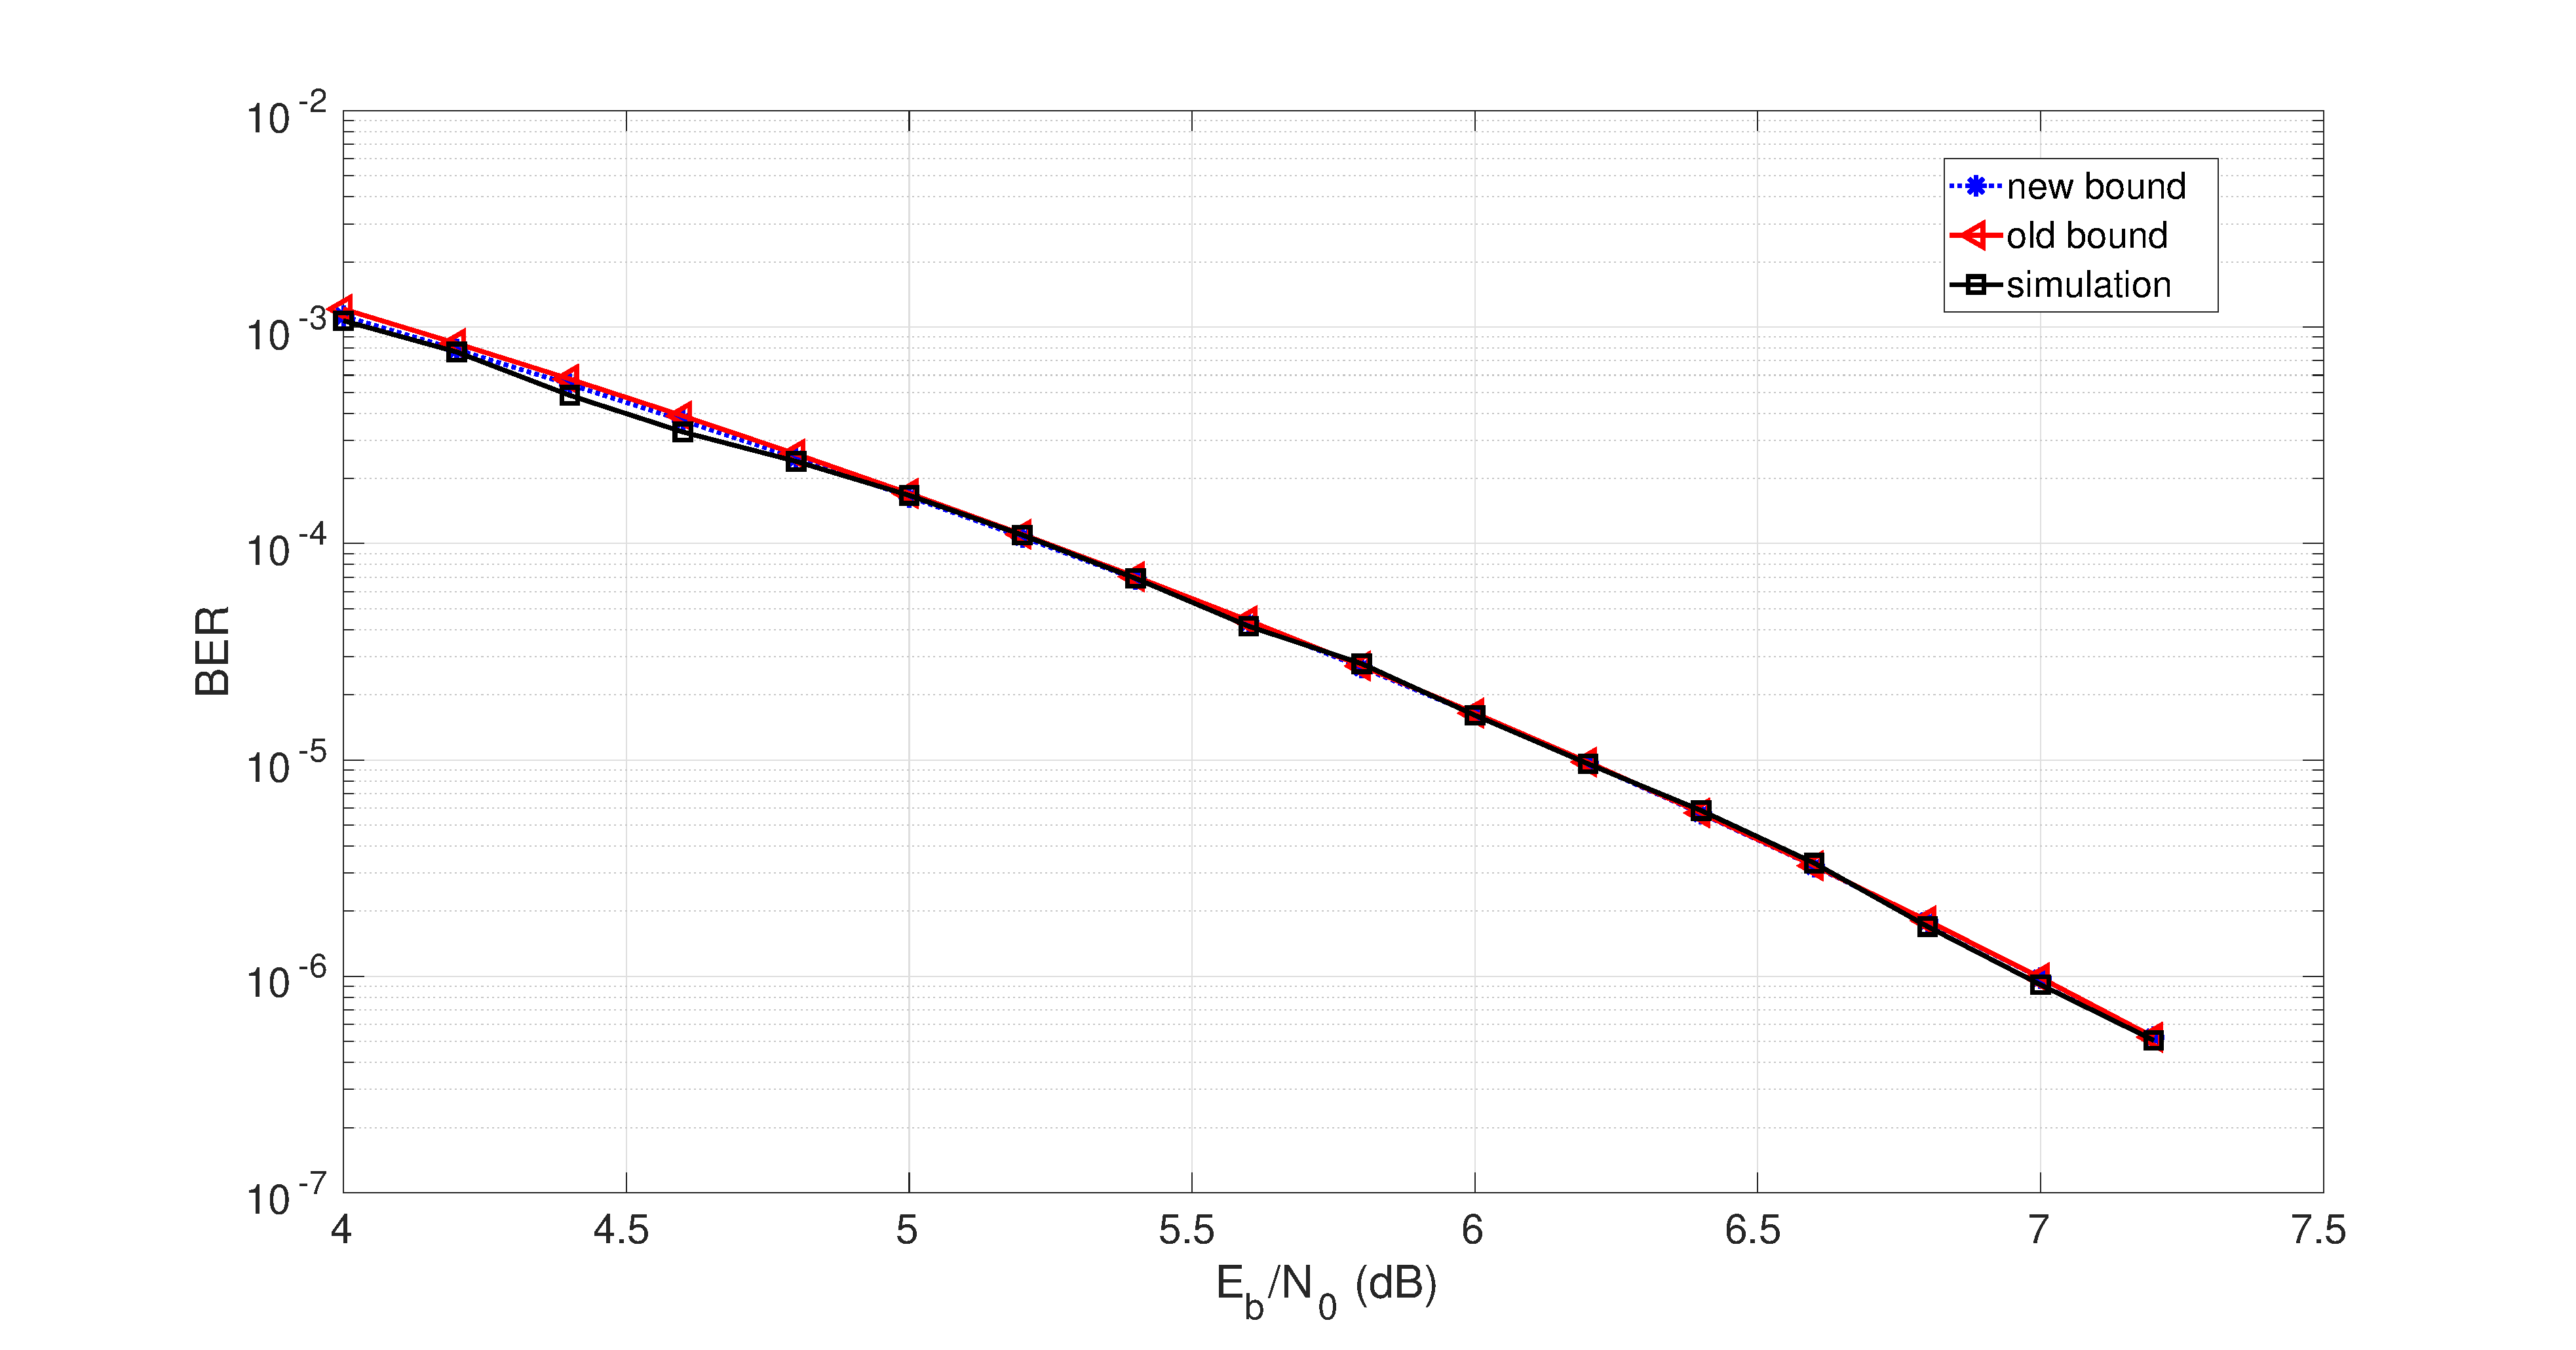
\includegraphics[width=0.5\textwidth]{./Images/RSC_5_7_lower_weights.eps}
		\caption{Old Bound vs New Bound vs Simulation for 5/7 RSC Code}
		\label{simFig1}
		\end{figure}
We observe that for both Fig. \ref{simFig1} and Fig. \ref{simFig2}, there is some difference between the new (novel method) bound and the old (transfer function) bound, but they tend to converge as $E_b/N_0$ increases. This suggests that codewords generated considering $b(x),~w_H(\bb)>3$ as well as codewords which have a parity-check sequence $h(x),~w_H(\bh)>3$ do not have much effect on the BER of the code as $E_b/N_0$ increases.

%The gap that is observed in the low $E_b/N_0$ regions is attributed to omitting codewords generated by the RTZ inputs of weight $w_H(\bb)=4$ as well as codewords with parity-check sequences $w_H(\bh)=4$ in our calculation of the new bound. 

%Fig. \ref{simFig4} and Fig. \ref{simFig5} are similar to  Fig. \ref{simFig1} and Fig. \ref{simFig2}, with the only difference being that codewords generated by the RTZ inputs of weight $w_H(\bb)=4$ as well as codewords with parity-check sequences $w_H(\bh)=4$ have been added in our calculation of the new bound. The new and old bounds match up and the accuracy of our bound is greatly improved.The simulation results also agree with the bounds as they also converge with the bounds.
\begin{figure}[h!]
\centering
		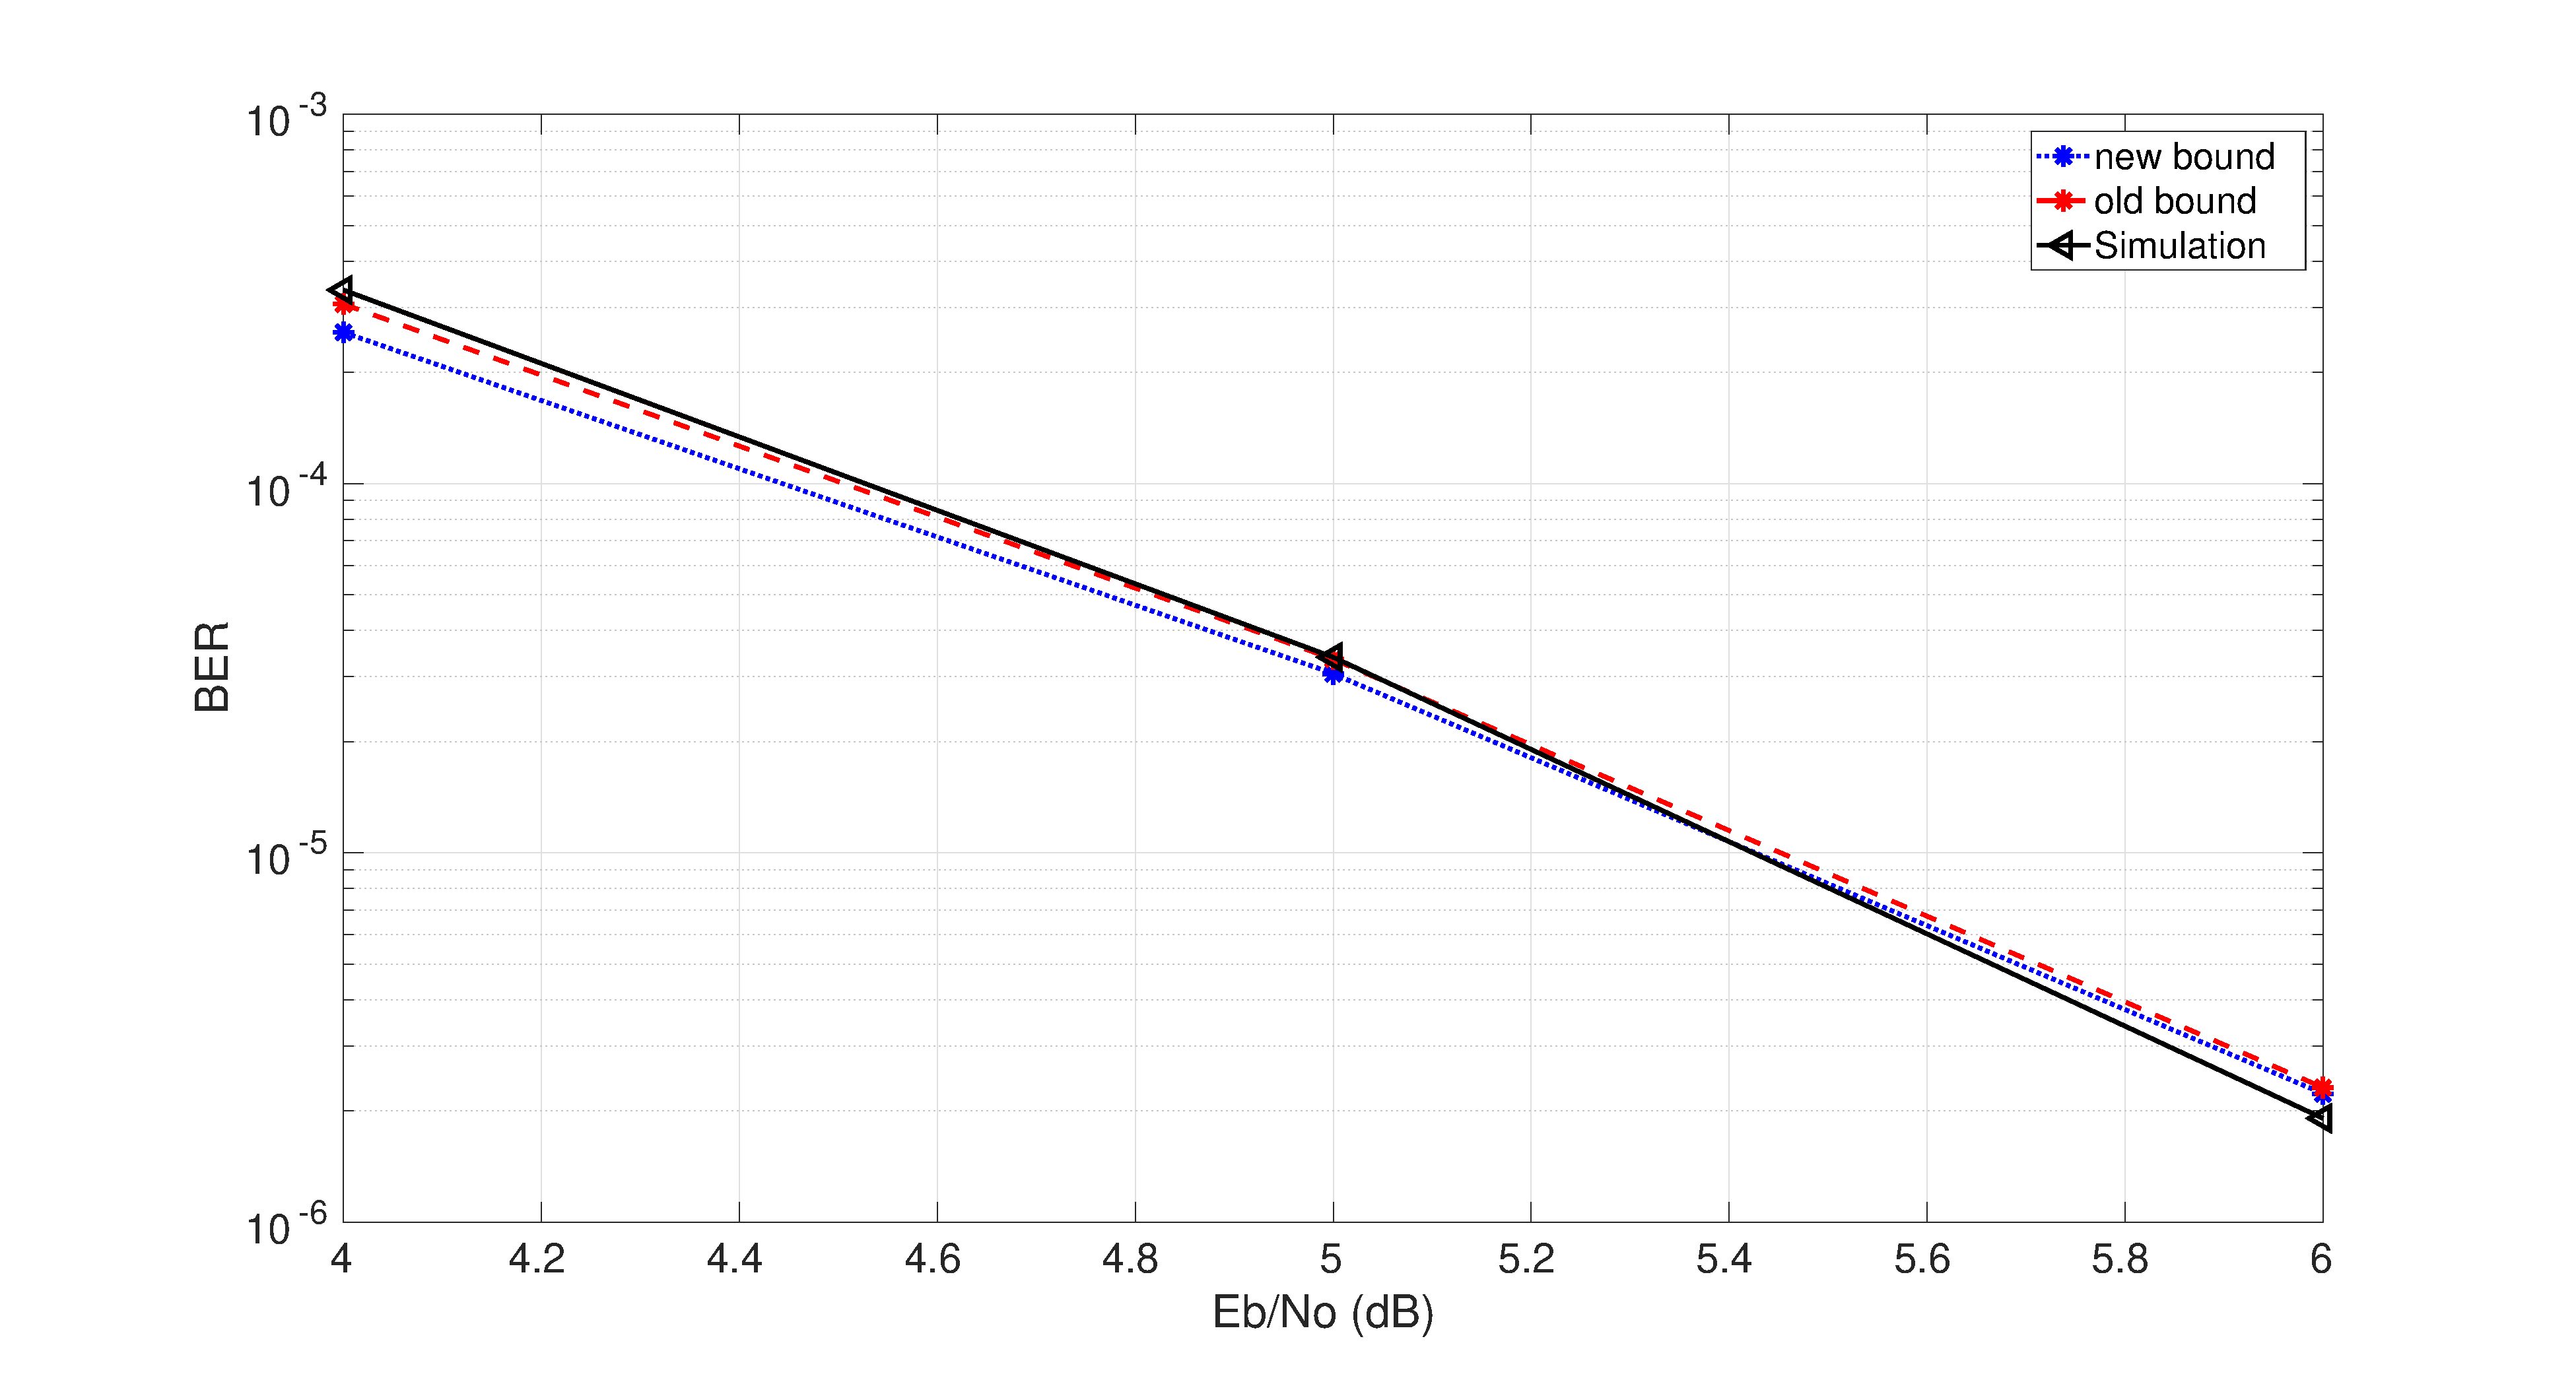
\includegraphics[width=0.5\textwidth]{./Images/RSC_37_21_v2.eps}
		\caption{Old Bound vs New Bound vs Simulation for 37/21 RSC Code}
		\label{simFig2}
		\end{figure}
However, in Fig. \ref{simFig3}, it is apparent that codewords generated by higher weight RTZs as well as those with parity-check sequences with weights $w_H(\bh)>3$ still dominate at higher $E_b/N_0$ values and need to be considered. As can be observed from the graph, there is a very distinct gap between the new bound and the old bound. Moreover, the bounds do not converge as $E_b/N_0$ increases. However, the old bounds and simulation results converge as the $E_b/N_0$ value increases. 
%In \ref{simFig3}, we observe that the old bounds and simulation results converge as the Eb/No value increases. However, there is a very distinct gap between the new bound and the old bound. Moreover, the bounds do not converge as the Eb/No increases. This means that we are missing vital elements in our approximation by not considering codewords generated by RTZ inputs of weight $w_H(\bb)>3$ as well as codewords with parity-check sequences $w_H(\bh)>3$. 

\begin{figure}[h!]
\centering
		\includegraphics[width=0.5\textwidth]{./Images/RSC_23_35_v3.jpg}
		\caption{Old Bound vs New Bound vs Simulation for 23/35 RSC Code}
		\label{simFig3}
		\end{figure}
		

%\begin{figure}[h!]
%\centering
%		\includegraphics[width=0.8\textwidth]{./Images/RSC_5_7_higher_weights.eps}
%		\caption{Old Bound vs New Bound vs Simulation for 5/7 RSC Code, with higher weights }
%		\label{simFig4}
%		\end{figure}
		
		
%		\begin{figure}[h!]
%\centering
	%	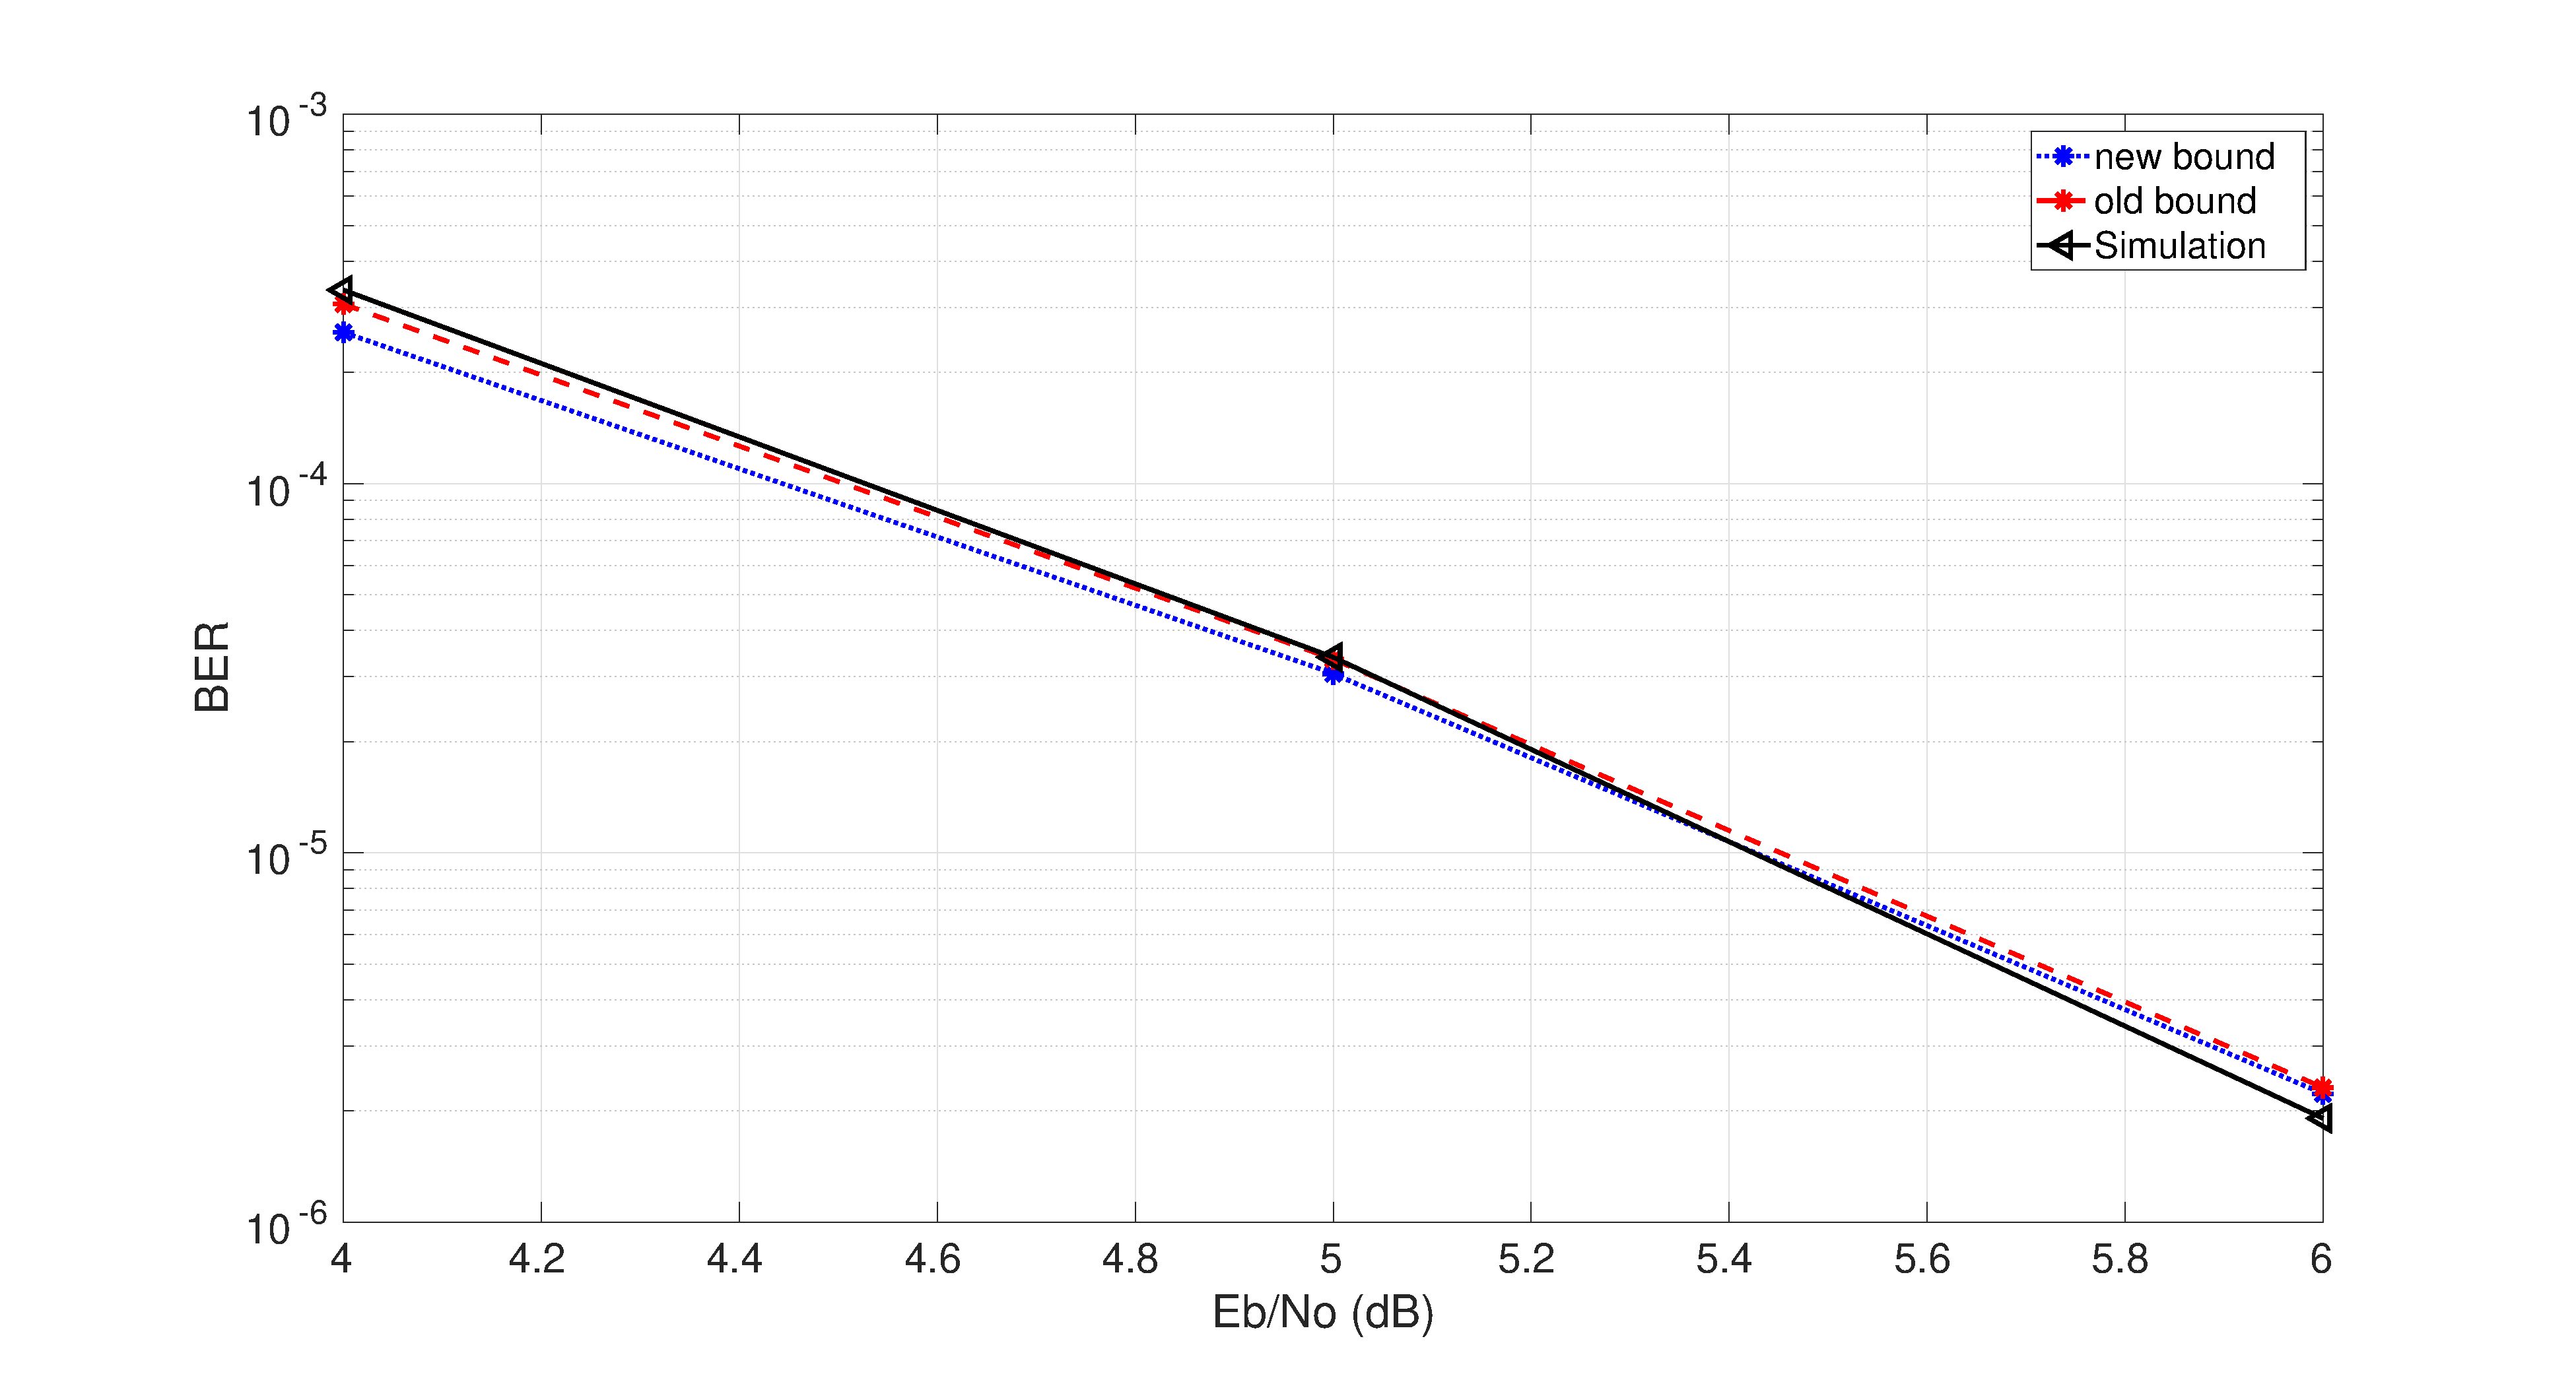
\includegraphics[width=0.5\textwidth]{./Images/RSC_37_21_v2.eps}
		%\caption{Old Bound vs New Bound vs Simulation for 37/21 RSC Code, with higher weights}
		%\label{simFig5}
		%\end{figure}



\newpage
\section{Conclusion}
\label{sec6}
%In this paper,we presented a novel low-complexity method for determining the distance spectrum of any RSC code which has the added benefit of revealing the structure of the Return-To-Zero (RTZ) inputs that make up the distance spectrum as well as their corresponding parity-check sequences. 
%%%%%%%%%%%%%%%%%%%%%%%%%%%
%We then go a step further and present a method  for deriving a general polynomial representation for both RTZ inputs and parity-check sequences with a Hamming weight of up to $4$ for any RSC code.
 %%%%%%%%%%%%%%%%%%%%%%
 
% Combining these two methods, we list the partial distance spectrum for selected RSC codes up to a cut-off weight $d_{\text{max}}$ and compare simulation results to the bounds obtained via our novel method and the regular method.

%In this paper, we presented a method for listing input message which produce codewords with low-weight parity bit sequences for a for a given $(n,k)$ RSC code. Compared to the Transfer function method, it has low complexity and provides more information about distance spectrum of the RSCC. Using a specially configured finite state machine, we can obtain a partial distance spectrum which we use to calculate an upper bound for the RSCC.  


In this paper, we presented a method for  obtaining the systematic and parity check component patterns of an RSC codeword given the RSC code and a cut-off weight, $d_{\text{max}}$.
%by focusing first on codewords with systematic components such that $2 \leq w_H(b(x)) \leq 3$, and then codewords with parity check components such that $2 \leq w_H(h(x)) \leq 3$. 
Compared to the transfer function method, it has low complexity and the knowledge of the pattern of $b(x)$ and $h(x)$ makes it a very useful for interleaver design. To validate our method, we compared the lower-bound obtained using our novel method with the lower-bound obtained via the transfer function as well as the simulation results for three RSC codes. Results show that whiles our method is sufficient for most RSC codes, considering codeword components with $w_H(b(x)), w_H(h(x)) =4$ in our approximation, might yield more accurate BER bounds.

\newpage
\begin{thebibliography}{99}
\bibitem{ref1}  C. Berrou, A. Glavieux and P. Thitimajshima, 
''Near Shannon limit error-correcting coding and
decoding: Turbo codes'', Proc. Intern. Conf. Communications (ICC), Geneva, 
Switzerland, pp. 1064-
1070, May 1993.
\bibitem{ref2} John G. Proakis, Masoud Salehi. ``Digital Communications'', 
Fifth Edition,Chapter 8, McGraw-Hill.
\bibitem{ref3} Todd K. Moon. ``Error Correcting Codes'',Chapter 12, John Wiley \& Sons.
\bibitem{ref4}Alain Glavieux, ``Channel Coding in Communication Networks: From Theory to Turbocodes'',\\ Chapter 3, John Wiley \& Son. 
\bibitem{ref5} Jing Sun, Oscar Y. Takeshita ''Interleavers for Turbo Codes Using 
Permutation Polynomials over Integer Rings'', IEEE Trans. Inform. Theory, vol. 51, 
pp. 101 - 119  Jan. 2005.
\bibitem{ref6} C. Berrou, Y. Saouter, C. Douillard, S. Kerouédan, and M. Jézéquel ``Designing Good Permutations for Turbo Codes: Towards a Single Model'',IEEE Communications Society 2004,pp.341-345

\end{thebibliography}



%\section{Upper Bound Comparison of both methods}
%\label{sec5}

%In order to confirm the validity of the proposed method, we compared the bit error rate (BER) upper bound the RSCC to results obtained through computer simulations. 

%There are a number of equations used to calculate the upper bound for the BER of a CC and these equations also apply to RSCC. For the case where the code is BPSK modulated and soft Viterbi decoding algorithm is used, the probability of bit error $P_b$ can be calculated using the equation below [3].

%\begin{equation}
%P_b \leq \frac{1}{k} \sum_{d=d_{\text{free}}}^{d_{\text{max}}} u(d) Q\Bigg( \sqrt{\frac{2dE_c}{N_0}}\Bigg)
%\label{eq5}
%\end{equation}
%where $u(d)=\sum_{w=1}^{\infty} w~ a(d,w)$,  $E_c/N_0$ is the Signal to Noise ratio for the transmitted codeword, $d_{\text{max}}$ is the largest value of $d$ used in the estimation of $P_b$ and $d_{\text{free}}$ is the free distance of the code. This equation require the knowledge of the distance spectrum of the RSCC and using the method described in the previous section,we obtain the partial distance spectrum for all input messages $b(x)$ of length $K=64$ which produce low-weight parity bits

%$h(x)$ where $w_H(\textbf{h})=2 ~\text{and} ~ w_H(\textbf{h})=4$.  We then use those terms with $d_{\text{max}}=8$ to calculate the probability of bit error using (\ref{eq5}). 

%For the simulation results we set $K=64$ and use a $5/7$ RSC encoder with tail-biting structure to encode the input messages. The codeword are BPSK modulated and transmitted over the AWGN channel. The soft Viterbi algorithm is used for the decoding and detection operation.

%\begin{figure}[h]
%\centering
%		\includegraphics[width=0.45\textwidth]{paperg2.png}
%		\caption{Simulation and Upper Bounds for $5/7$ RSCC}
%		\label{fig3}
%		\end{figure}
		
%		The simulation results are compared with the upper bound in Figure \ref{fig3}. 
%	We deduce that it is possible to estimate the performance of the RSC code by the upper bound obtained using our novel method. The difference between the upper bound and the simulation results is $1.3730 \times 10^{-4}, 2.9960 \times 10^{-5},2.2800 \times 10^{-6}, 1.5668^{-7}$ for $E_b/N_0$ (dB) values of $4,5,6~\text{and}~7$ respectively. 
%We observe that for $E_b/N_o$ value of  $6$ dB, the upper bound is x dB away from the simulation results whiles it is y dB from the simulation results at an $E_b/N_o$ value of  $6$ dB




%\end{enumerate}

\end{document}